%%%%%%%%%%%%%%%%%%%%%%%%%%%%%%%%%
%% Ersetzen Sie in den folgenden Zeilen die entsprechenden -Texte-
%% mit den richtigen Werten.
\documentclass[course=erap]{aspdoc}
% \newcommand{\theGroup}{IhreGruppennummer} % Beispiel: 42
% \newcommand{\theNumber}{IhreProjektnummer} % Beispiel: A123
\author{Tobias Hanl \and Jonas Jürß \and Tobias Wothge}
\date{Wintersemester 2019/20} % Beispiel: Wintersemester 2018/19
%%%%%%%%%%%
\usepackage{float}
\usepackage{amssymb}
\usepackage{pgfplots}
\pgfplotsset{compat=1.15}
\usepackage{longtable}
\usepackage{subcaption}
\usepackage{xcolor}

% Diese Zeile bitte -nicht- aendern. -- Tja, trotzdem geschehen :D
\title{Parallele Evolutionssimulation}


\begin{document}
\maketitle


\setcounter{tocdepth}{2}
\tableofcontents


\newpage


\section{Einleitung}
Die Natur hat viele spannende und interessante Aspekte zu bieten. Seien es die Vielfalt an Pflanzen und Lebewesen oder auch die beeindruckenden Landschaften -- wie beispielsweise die Alpen --, die überall auf der Welt zu finden sind. Eines aber haben diese Aspekte alle gemeinsam: Sie sind einmalig! Vor allem der Artenreichtum in der Tier- und Pflanzenwelt ist beeindruckend. Er ist so groß, dass bis heute noch viele Spezies unentdeckt bleiben, obwohl immer wieder Neue gefunden werden. Dies liegt vor allem daran, dass viele Arten über die Zeit aussterben, aber wiederum auch viele Neue entstehen. Diese sogenannte Evolution ist eine der spannendsten Themen der Natur überhaupt. Durch sie passen sich Lebewesen immer mehr ihrer aktuellen Umgebung an und können so selbst in Gebieten überleben, wo andere Arten nach kurzer Zeit aussterben würden. Daher ist es nicht abwegig, dass man versucht diese Evolution genauer zu verstehen und daher Modelle hierfür entwickelt, in denen man die Evolution simulieren kann. So ein Modell soll nun auch in diesem Projekt entwickelt werden.

Dafür wird im Folgenden eine Simulation konzipiert, welche ein eigens entwickeltes Modell umsetzt. Diese Simulation soll als ausführbares Programm implementiert werden und es so ermöglichen, die Evolution für die unterschiedlichsten Umstände berechnen und beobachten zu können. Zudem wird die Simulation anschließend parallelisiert, um rechenintensive Abschnitte performanter zu machen. Genau dieser Prozess wird nun in den folgenden Seiten der Ausarbeitung vorgestellt und detaillierter erklärt werden.


\section{Problemstellung und Spezifikation}
Das Fundament für die Simulation bildet eine abstrakte Welt. Auf ihr sollen sich später Lebewesen bewegen, dort Nahrung finden und mit anderen Lebewesen interagieren können. Das Hauptaugenmerk wird hierbei grundsätzlich auf der Evolution liegen. Das heißt, es ist primär von Interesse, wie sich über die Zeit unterschiedlichste Spezies entwickeln, welche dann auch gewisse Merkmale -- wie zum Beispiel unterschiedliche Überlebensstrategien -- ausbilden werden. Dabei soll diese Welt eine möglichst gute Approximation der realen Welt abgeben. Somit werden sich nach Möglichkeit ähnliche Verhaltensmuster von Lebewesen entwickeln, wie sie auch aus der Natur bekannt sind. Natürlich wird die Simulation nur auf die grundlegendsten Aspekte beschränkt sein, da die Evolution doch ein komplexes und schwierig simulierbares Konzept darstellt.


\subsection{Die Welt}
\label{subsec:die-welt}
Wie im vorherigen Absatz erwähnt, soll die Welt nur einer abstrakten Näherung der realen Welt entsprechen. Sie muss somit nicht den bekannten Strukturen und Gesetzen unserer Erde entsprechen. Daher wird aus Gründen der Einfachheit die Welt in der Simulation ein Rechteck sein, welche an den Rändern offen ist. Das heißt, die Ränder stellen keine undurchdringliche Begrenzung dar, sondern alles kann sich über diese hinwegbewegen. Andererseits gibt es dann keine Möglichkeit mehr, auf die Welt zurückzukehren. Der Bereich hinter den Rändern soll somit einen unendlich tiefen Abgrund darstellen. Somit ergibt die Welt auch keine Kugel (wie unsere Erde), bei der man sich nach einer Umkreisung wieder am Startpunkt befindet.

Allerdings soll die Welt nicht nur eine einfache Fläche darstellen, die keinen Inhalt besitzt, sondern es wird auf dieser Fläche zusätzlich eine Struktur geschaffen werden, durch welche die Welt vielschichtiger wird. Durch diese Struktur sollen Umgebungen geschaffen werden, welche dann unterschiedliche Merkmale gegenüber anderen Umgebungen aufweisen werden. Dafür wird nun das sogenannte \emph{Terrain} eingeführt, welches genau diese Struktur erzeugt.

Das Terrain zerteilt hierbei die Welt in viele gleich groß dimensionierte, kleine Quadrate, im Folgenden \emph{Tiles} genannt. Jedes Tile ist dabei von einem der vier folgenden Typen: Wasser, Sand, Grass oder Stein. Dabei sollen diese Typen zufällig, aber trotzdem realistisch (z.B. Sand am Wasser, zusammenhängende Flächen vom gleichen Typus) auf die Tiles verteilt werden. Hieraus ergibt sich somit eine Landschaft, welche die Welt einzigartig macht und dabei besondere Umgebungen schafft.


\subsection{Food-Entities}
Zusätzlich zur Struktur befinden sich auch Objekte (\emph{Entities}) auf der Welt. Eine Art dieser Objekte sind die sogenannten \emph{Food-Entities}. Diese stellen Nahrung dar, welche sich auf der gesamten Welt verteilt befindet. Hierbei wird nicht zwischen verschiedenen Arten von Nahrung unterschieden. Eine Ausnahme stellt nur der "`Boarisch Mode"' dar (siehe Abschnitt \ref{sssec:exec-params}, unten). Über die Energieaufnahme hinaus hat es in der Simulation keine Vorteile ein Entity zu fressen.

Vor allem müssen die Food-Entities aber auch eine "`nachwachsende"' Ressource sein. Das heißt, es werden über die Zeit weitere Food-Entities auf der Welt verteilt werden. Dies verhindert, dass irgendwann über die Zeit die Nahrung ausgeht und keine mehr nachkommt. Die Nahrung soll somit auf der Welt höchstens knapp werden. Trotzdem dürfen die Food-Entities aber auch nicht unendlich lange existieren. Die Food-Entities besitzen daher eine Haltbarkeitszeit, nach deren Ablauf sie keine Energie mehr liefern können und daraufhin verschwinden. Hierdurch soll einem Überangebot von Nahrung -- und damit auch Energie -- auf der Welt entgegengewirkt werden.


\subsection{Living-Entities}
Als letztes Element der Simulation fehlen nun noch die Lebewesen, welche auf dieser Welt beheimatet sind. Dies sind die sogenannte \emph{Living-Entities}, die sich auf der Welt bewegen und dabei über Generationen hinweg weiterentwickeln können. Sie werden somit die eigentliche Evolution in der Simulation durchlaufen. Hierfür besitzen die Living-Entities einige Merkmale und Attribute, so dass sich potenziell möglichst viele unterschiedliche Arten beziehungsweise Spezies von Lebewesen entwickeln können. Diese Merkmale und Attribute sollen nun im Folgenden vorgestellt und genauer erläutert werden.


\subsubsection{Das Gehirn}
Wichtigstes Merkmal der Living-Entities ist es, dass sie \emph{frei} Entscheidungen treffen können. Dies ist für die Evolution essenziell, da auch in der Natur viele Lebewesen die Möglichkeit haben, durch ein Gehirn \emph{eigenständig und frei} Entscheidungen zu fällen. Beispielsweise können diese Entscheidungen über Leben oder Tod entscheiden und nehmen somit einen wichtigen Einfluss auf die Entwicklung einer Spezies. Daher sollen auch die Living-Entities in der Simulation ein eigenes Gehirn bekommen, mit welchem sie frei Entscheidungen treffen können. Somit wird es notwendig sein, eine möglichst gute \emph{künstliche Intelligenz (KI)} zu entwickeln, welche genau dies möglichst realistisch umsetzt.


\subsubsection{Energiehaushalt und Nahrungsquellen}
Das wichtigste Attribut, neben dem Gehirn, ist die Energie der Living-Entities. Diese entscheidet darüber, ob ein Entity tot (\(\leq 0\)) oder lebendig (\(> 0\)) ist. Wenn das Living-Entity tot ist, wird es aus der Welt entfernt. Es verbraucht seine Energie die ganze Zeit über, solange es lebendig ist. Dafür besitzt jedes Entity, je nach Größe, einen festgelegten Grundumsatz an Energie. Zusätzlich verliert es mehr Energie, wenn es sich bewegt, wobei dies einzig von der Geschwindigkeit des Entities abhängt. Je schneller es sich auf der Welt bewegt, desto mehr Energie verbraucht es.

Somit sollte ein Entity seine Energie gut einteilen, um möglichst lange überleben zu können. Größter Energielieferant ist hierfür Essen (Food Entities). Allerdings ist es allen Entities auch freigestellt, fremde (nicht der eigenen Spezies zugehörige) Entities anzugreifen, falls diese auf den gegebenen Untergrund sichtbar sind. Falls sie den Kampf gewinnen -- ausschlaggebend ist hier die Größe der Kontrahenten --, bekommen sie die gesamte Energie des gestorbenen, fremden Entities übergeben. Verlieren sie jedoch den Kampf, weil sie kleiner sind, so stirbt das Entity selbst. Zusätzlich kann jedes Entity auch einen Teil seiner Energie freiwillig abtreten und diese einem Freund (eigene Spezies) geben, so dass dieser länger überleben kann. Jedoch kann ein Living-Entity andere Entities (Nahrung wie auch Lebewesen) nicht über die gesamte Welt hinweg sehen. Es besitzt daher einen festgelegten \emph{Sichtradius} innerhalb dessen das Entity Andere überhaupt erst wahrnehmen kann.


\subsubsection{Fortpflanzung}
Ein weiteres wichtiges Merkmal der Living-Entities ist die Möglichkeit zur Fortpflanzung. Hierfür wird ein neues Kind-Entity erstellt, welches mit einer gewissen Wahrscheinlichkeit ein leicht verändertes Verhalten aufweist. Das Kind soll also eine Mutation des Eltern-Entities sein und daher leicht veränderte Merkmale aufweisen, welche sich unter Umständen als besser herausstellen. Living-Entities können sich nur vermehren, wenn sie dafür genug Energie besitzen. Einen Sexualpartner (anderes Living-Entity) brauchen sie für die Fortpflanzung hingegen nicht. Daher wird auch nicht zwischen Geschlechtern differenziert.

Wichtig ist es noch, anzumerken, dass in der Fortpflanzung und der daraus resultierenden Mutation im Kind-Entity auch die eigentliche Evolution liegt. Die Entities selbst sollen sich daher nicht weiterentwickeln. Dies schließt beispielsweise mit ein, dass die Gehirne der Entities nicht trainiert, sondern (indirekt) über die Evolution verbessert werden sollen.

Indessen wird die Fortpflanzung noch weiter gesteuert, da sich Entities nicht willkürlich die ganze Zeit vermehren können sollen, sobald sie genug Energie besitzen. Ein \emph{Cooldown} (Counter) bestimmt hierfür, wie lange das Entity warten muss, bis es sich frühestens wieder vermehren kann. Falls das Entity zu wenig Energie besitzt, wenn der Cooldown ausläuft, darf es sich erst vermehren, sobald es genug Energie hat. Nach der Fortpflanzung wird der Counter wieder zurückgesetzt.


\subsubsection{Agilität im Wasser und auf Land}
Damit sich ein Entity auch zusätzlich noch an seine Umgebung anpasst, besitzt jedes Entity eine Wasseragilität. Diese entscheidet darüber, wie schnell sich ein Entity in Wasser bewegen kann. Allerdings läuft diese Agilität gegensätzlich zur Fähigkeit, sich schnell auf Land fortbewegen zu können. Konkret bedeutet dies: je höher die Wasseragilität, desto langsamer bewegt sich das Entity auf Land (Sand, Grass und Stein). Jedoch erlaubt eine geringere Wasseragilität sich schneller auf Land zu bewegen. Damit sollen Entities einen Vorteil gegenüber anderen haben, die eine schlechtere Agilität als sie selbst in der aktuellen Umgebung besitzen. Daher sollte ein Entity beispielsweise darauf achten, Wasser zu meiden, wenn es eine schlechte Wasseragilität hat. Dies gilt auch für die gegensätzliche Konstellation.


\subsection{Visualisierung der Simulation}
\label{subsec:visualisierung-simulation}
Um die Simulation während der Ausführung beobachten zu können, muss es möglich sein, sie zu visualisieren. Hierfür wird die Welt in ihrer aktuellen Größe in einem Fenster dargestellt. Die Struktur der Welt und die einzelnen Elemente (Living- und Food-Entities) werden in dieses Fenster eingezeichnet. Dieser \emph{Render-mode} bietet somit eine Schnittstelle zwischen dem Beobachter und der eigentlichen Simulation an. Allerdings muss es auch möglich sein, die Simulation ohne eine Anzeige auszuführen. Dies ist vor allem für Systeme interessant, welche kein eigenes Display besitzen. Umgesetzt wird dies durch den sogenannten \emph{Hidden-mode}. In diesem wird es dafür anderweitige Möglichkeiten geben (z.B. über die Kommandozeile) die Simulation zu beobachten. Hierbei muss es aber immer möglich sein, zwischen den beiden Modi während der Ausführung zu wechseln. Sollte die Simulation beispielsweise über Stunden oder auch Tage hinweg ausgeführt werden, kann es wünschenswert sein, diese für die Ausführungszeit im "`Hintergrund"' weiter laufen zu lassen. Hierbei ließe sich das Fenster für diese Zeit verstecken. Zusammenfassend unterstützt die Simulation somit zwei verschiedene Modi, in denen diese beobachtet werden kann -- jeweils passend für die aktuellen Umstände.


\newpage
\section{Lösungsfindung}
\label{sec:lösungsfindung}
Nachdem das Modell beschrieben und die Anforderungen an die Simulation spezifiziert wurden, sollen jetzt der konkrete Lösungsweg, sowie die konzeptionelle Gestaltung der Implementierung aufgezeigt werden. Dafür werden im Folgenden, für die verschiedenen Anforderungen, konzeptionelle Lösungen aufgezeigt und genauer erläutert.


\subsection{Neuronale Netze zur Verhaltenssimulation}
\label{subsec:neuronale-netze}
Einen wichtigen Teil der Simulation stellt das Verhalten der Lebewesen dar. Um dieses möglichst realistisch zu gestalten, hat jedes Lebewesen ein neuronales Netz, welches Eingabewerte zur Entscheidungsfindung gewichtet und so bestimmte Ausgabewerte erzeugt, welche die Handlungen festlegen. Dieses Konzept ist eine stark vereinfachte Abstraktion des Gehirns, in welchem für Denkvorgänge entscheidend ist, ob ein Impuls stark genug ist, um von einer Nervenzelle weitergegeben zu werden.


\subsubsection{Funktionsweise}

In der Simulation hat jedes Lebewesen ein einfaches neuronales Netz. Jedes Neuron einer Ebene erhält seinen Wert, indem es die Ausgabe jedes Neurons der vorherigen Ebene mit einem Faktor gewichtet, die Werte summiert und eine Konstante addiert. Durch Anwendung einer sogenannten Aktivierungsfunktion wird sichergestellt, dass das Ergebnis in einem kleinen Intervall -- beispielsweise $(-1,1)$ -- liegt. So kann es nicht übermäßig groß oder klein werden und somit das Ergebnis folgender Neuronen durch einen einzelnen Wert unverhältnismäßig ändern. Prinzipiell lässt sich also sagen, dass eine Entscheidung getroffen wird, indem die Eingaben gewichtet werden. In einem einfachen Beispiel, welches nur aus einer Ein- und einer Ausgabeebene besteht, könnte das Neuron für die Rotation den Winkel zur Nahrung mit 1 und alles andere mit 0 gewichtet (siehe Abbildung \ref{fig:nn-example}). Das Entity würde sich dann immer in Richtung der nächsten Nahrung bewegen.

\begin{figure}[H] %the tikz graphic didn't compile in this specific setup :(
    \centering
    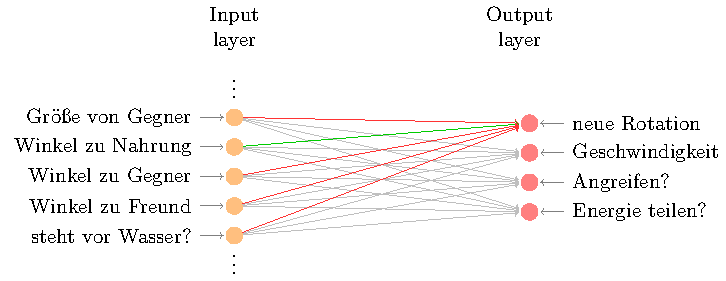
\includegraphics[width=.9\textwidth]{res/nnexample.pdf}
    \caption{Vereinfachtes Beispiel eines neuronalen Netzes}
    \label{fig:nn-example}
\end{figure}

\subsubsection{Aufbau}
Tatsächlich besteht das neuronale Netz in der Simulation aus drei Ebenen. Die zusätzliche, sogenannte "`Hidden Layer"' ermöglicht das Treffen etwas komplexerer Entscheidungen. So könnte beispielsweise eines der Neuronen in dieser Ebene einen "`Gefährdungsgrad"' angeben, indem es Werte wie Distanz und Größe des Gegners gewichtet. Dieser wäre dann eine Eingabe für die Ausgabeebene, in welcher beispielsweise die Geschwindigkeit diese Gefährdung hoch gewichten könnte -- auf einer Flucht würde das Lebewesen sich also so schnell wie möglich bewegen. Gleichzeitig könnte das Teilen von Energie die Gefährdung negativ gewichten und somit dafür sorgen, dass während der Flucht die komplette Energie dem Lebewesen selbst zur Verfügung steht.

Hierbei ist anzumerken, dass die versteckten Neuronen selten einen Wert angeben, dessen Bedeutung so einfach logisch nachvollziehbar ist. Die Anzahl der versteckten Ebenen und deren Neuronen kann beliebig gewählt werden. Allerdings wird es durch jeden neuen Wert unwahrscheinlicher, dass zufällige Werte einen positiven Effekt haben (siehe \ref{sssec:nn-problem}). In Kombination mit der steigenden benötigten Rechenleistung und dem zusätzlichen Aufwand beim Versenden sowie dem Umstand, dass die Komplexität sinnvoller Verhaltensmuster in einer so einfachen Simulation beschränkt ist, stellen sich mehr Ebenen oder Neuronen allerdings als nicht zielführend heraus.

In Abbildung \ref{fig:neural-net} ist der finale Aufbau des Netzes zu sehen. Im Wesentlichen können also in jedem \emph{Tick} vier Entscheidungen getroffen werden: die Bewegungsrichtung, die Bewegungsgeschwindigkeit (auf Kosten eines höheren Energieverbrauchs), die Entscheidung, ob Energie geteilt werden soll, sofern sich ein ähnliches Lebewesen ("`gleiche Spezies"') in der Nähe befindet, sowie die Frage, ob ein Lebewesen einer anderen Spezies angegriffen werden soll, sofern sich eines in der Nähe befindet.

\begin{figure}[H]
    \centering
    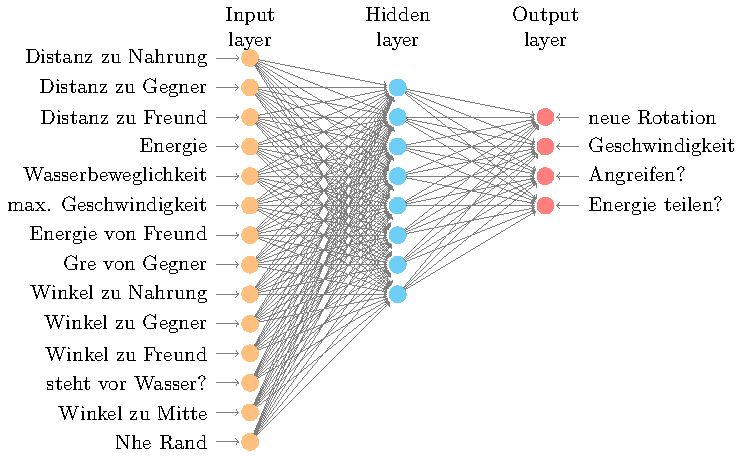
\includegraphics[width=.85\textwidth]{res/neuralnet.pdf}
    \caption{Genauer Aufbau des neuronalen Netzes}
    \label{fig:neural-net}
\end{figure}

\subsubsection{Normalisierung der Werte}
Ein wichtiger Teil bei der Verwendung neuronaler Netze ist die sinnvolle Wahl und Normalisierung von Ein- und Ausgabewerten. So werden beispielsweise keine kartesischen Koordinaten im neuronalen Netz verwendet, sondern Polarkoordinaten. Grund hierfür ist die höhere, semantische Aussagekraft. Während beispielsweise die Distanz direkte Relevanz für eine Entscheidung hat, ist das für x- und y-Differenz nicht der Fall. Hier müssten erst einige Neuronen verwendet werden, um einen ähnlich aussagekräftigen Wert zu erlangen. Entsprechend könnte beispielsweise keine separate Entscheidung zur Geschwindigkeit getroffen werden, diese wäre immer von der errechneten x- und y-Differenz abhängig. Es ergäbe sich ein neuronales Netz, welches weniger sinnvolle Entscheidungen träfe. In diesem Rahmen ist außerdem zu erwähnen, dass bei den angegebenen Werten stets das Lebewesen selbst als Mittelpunkt des Koordinatensystems gewählt wird. Erneut kann leicht nachvollzogen werden, dass beispielsweise der Abstand eines Gegners vom Lebewesen selbst eine höhere semantische Bedeutung hat, als der Abstand vom Mittelpunkt der Welt. Außerdem kann so beispielsweise einfach der Winkel zu einem Objekt mit eins gewichtet werden, um sich in dessen Richtung zu bewegen.

%Neben dem geänderten Ein- und Ausgabeformat für Koordinaten, mögen zunächst einige Eingabewerte ins Auge stechen. So wäre die Wasseragilität nicht zwingend nötig, da diese bei einer Spezies selbst nur bei der Vererbung mutiert, wie auch das neuronale Netz selbst. Es würde also zunächst reichen, dass Wasserlebewesen auf dem Land einen evolutionären Nachteil haben und sich somit dahingehend entwickeln, dass sie sich eher nicht in Richtung Land bewegen. Der zusätzliche Eingabeparameter ermöglicht eine Abstraktion. Lebewesen können sich bevorzugt zu ihrem präferierten Untergrund bewegen, anstatt fest Wasser oder Land zu bevorzugen. So können sich leichter Wasserlebewesen auf Landlebewesen und umgekehrt entwickeln, wenn deren Wasseragilität mutiert. Außerdem erleichtert es das Vortrainieren der Netze, da dies allgemein stattfindet, bevor die konkreten Attribute bekannt sind (siehe \ref{sssec:nn-problem}).
%Darüber hinaus werden vorberechnete Werte wie der Winkel zur Mitte oder die Distanz zum Rand als Parameter gewählt, um die Entscheidung zu erleichtern, sich nicht aus der Welt zu bewegen und somit zu sterben.

\subsubsection{Lernen}
Eine Herausforderung bei diesem Projekt war, dass die neuronalen Netze der Lebewesen nicht trainiert werden. Dies wäre nur sehr kompliziert zu verwirklichen, da nicht ohne weiteres bei jeder Handlung evaluiert werden kann, ob diese gut oder schlecht war. Das Verwenden einer simplen Heuristik - wie etwa die schnelle Aufnahme von Energie - wäre mittels eines sogenannten Rekurrenten Neuronalen Netzes, bei welchem die Ausgaben der letzten Berechnung als zusätzliche Eingaben dienen, zwar möglich, könnte allerdings komplexere Verhaltensmuster unterbinden, da gegebenenfalls nur das schnelle Sammeln von Nahrung "`belohnt"' würde, nicht aber der sparsame Umgang oder das Teilen mit anderen.

Darüber hinaus müsste - würden die Netze trainiert - die Evolution über deren Struktur stattfinden, was zwar näher an der Realität, dafür jedoch ebenfalls nur schwer sinnvoll zu implementieren wäre.
Daher bestand der Ansatz zunächst darin, die neuronalen Netze wie alle anderen Attribute zufällig zu initialisieren und bei Fortpflanzung nur leicht zu verändern, sodass sinnvolle Gewichtungen durch Evolution entstehen.


\subsubsection{Aussterben zu Beginn aufgrund wenig sinnvoller Initialisierung}
\label{sssec:nn-problem}
Während die ursprüngliche Strategie mit wenigen Neuronen - beispielsweise nur der nächsten Nahrung als Ein- und der Bewegungsrichtung als Ausgabe - funktioniert, stellt sie sich beim Hinzufügen weiterer Entscheidungsmöglichkeiten als problematisch heraus. Die große Anzahl an möglichen Kombinationen macht eine überlebensfähige Initialisierung unwahrscheinlich, sodass in vielen Durchläufen alle Lebewesen aussterben, bevor durch Evolution eine ausreichende Anpassung erfolgen kann. Ansätze wie eine bessere Initialisierung der Gewichte (nach Xavier) oder die Verwendung Rekurrenter Netze bringen zwar Verbesserung, jedoch nicht im benötigten Ausmaß.

Um bereits zu Beginn überlebensfähige Lebewesen sicherzustellen, werden die Gewichtungen daher nun zufällig aus einer Menge vortrainierter Netze gewählt. Der Ansatz ist hier, das Verhalten in einem bestimmten Szenario festzulegen, alles andere jedoch offen zu lassen, sodass dennoch unterschiedliche Verhaltensmuster entstehen können.


\subsection{Parallelisierung}
Viele Operationen in der Simulation sind sehr rechenintensiv. Dazu zählen beispielsweise die Denkprozesse der Living-Entities, welche durch Matrix- bzw. Vektoroperationen (wie dem Skalarprodukt) implementiert sind und auf größeren Datenmengen agieren. Auch das Rendering ist rechenintensiv, da hier alle Texturen zuerst berechnet und danach übereinander gelegt werden müssen. Folglich können diese Operationen dazu führen, dass die Simulation auf einem einzelnen Rechner mit nur einem Thread sehr langsam läuft, da ein Tick viel Rechenzeit benötigt. Somit würde die Simulation oft blockieren und nur träge einen Fortschritt zeigen. Um dieses Problem zu lösen, soll die Simulation parallelisiert werden. Die rechenintensiven Aufgaben können so besser verteilt und die Simulation in Folge performanter ausgeführt werden.


% TODO: Ggf. Verlinkung auf Abschnitt zur Performance und Ergebnissen hinzufügen, um diesen Abschnitt besser zu belegen!!!
\subsubsection{Rechenintensive Abschnitte}
Hauptproblem für die Performance der Simulation ist die KI. Für diese müssen für jedes \emph{einzelne} Entity sehr viele aufwendige Rechenoperationen durchgeführt werden. Hierbei werden vor allem Matrixoperationen benötigt. Genaueres dazu im Abschnitt \ref{subsec:neuronale-netze}. Diese werden wiederum in jedem Tick ausgeführt und benötigen somit sehr viel Rechenleistung. Für kleine Zahlen von Entities ist dies noch erträglich. Allerdings summiert sich dies für alle weiteren Entities auf und es wäre somit von Vorteil diese Berechnungen auf mehrere Prozesse bzw. Threads aufteilen zu können, damit die Simulation trotzdem performant läuft.

Zudem spielt auch die Weltgröße eine wichtige Rolle. Auf einer großen Welt haben mehr Entities Platz, als auf einer kleineren. Somit befinden sich im Mittel auf einer solchen Welt auch mehr Entities. Wie aus dem vorherigen Absatz erkennbar, ist die Entity-Zahl eine wichtige Größe für die Gesamtperformance der Simulation. Somit wird es nötig sein, eine sehr große Welt in kleinere Welten aufbrechen zu können und diese parallel berechnen zu lassen. Folglich müsste sich jede Teilwelt um weniger Entities kümmern und würde somit weniger Rechenleistung benötigen. Die Simulation wäre in Folge performanter.

Falls die Simulation noch zusätzlich in einem Fenster angezeigt werden soll, benötigt das Rendering, je nach Weltgröße und Entity-Zahl, nochmal zusätzlich Rechenleistung. Eine Aufteilung der Welt auf kleinere Teilwelten würde in diesem Fall somit auch eine Leistungssteigerung bewirken, da nur noch eine kleinere Welt mit weniger Details gerendert und angezeigt werden müssten.


\subsubsection{Parallelisierung mittels MPI}
Hauptsächlich sollen diese Probleme durch das \emph{Message Passing Interface (MPI)} gelöst werden. Durch dieses wird es möglich sein, die gesamte Welt auf beliebig viele Rechner (\emph{Nodes}) im gegebenen Cluster aufteilen zu können. Hierfür bekommt jeder Node genau eine Teilwelt zugewiesen, so dass alle Rechner zusammen wieder die gesamte Welt bilden. Allerdings wird auf jeder Node nur ein einzelner Prozess für die Simulation ausgeführt, unabhängig von den verfügbaren Kernen.

Nach der Spezifikation muss sichergestellt werden, dass sich die Living-Entities auf der \emph{gesamten} Welt bewegen können. Es muss für diese also so aussehen wie als gäbe es keine Grenzen zwischen den Teilwelten. Folglich sind die Nodes gezwungen untereinander zu kommunizieren, damit Living-Entities weitergereicht werden können. Gerade hierfür eignet sich MPI bestens, da es für genau solche Situationen ein leicht verständliches und trotzdem sehr praktisches Interface bietet.

Die Kommunikation zwischen den Nodes wird nun wie folgt stattfinden. Um selbst bei einer sehr hohen Anzahl von Nodes die Simulation gut skalieren zu können, kommunizieren die Nodes \emph{eigenständig} untereinander. Das heißt, es wird keinen Root Node geben, der alle Nachrichten von den Nodes bekommt und diese dann daraufhin an die richtigen Nodes verteilt. Dies würde zu einem \emph{Bootle-Neck} am Root Node führen, da die Nodes warten müssten, bis alle Nachrichten angekommen und danach vom Root wieder ausgesendet wurden. Stattdessen soll jeder Node wissen, welche Nodes angrenzende Teilwelten an die eigene verwalten, weil nur von diesen Nachrichten (Living-Entities) kommen können. Die Teilwelten müssen dementsprechend groß genug sein.

% [ANMERKUNG]: Dies beschreibt ein wenig den MaiMUC. Soll dies noch rein?
% Vor allem ist aber die Parallelisierung mit MPI für den MaiMUC wichtig. Dieser besteht aus mehreren Raspberry Pi's, die jeweils ein eigenes Display besitzen. Auf diesem soll es möglich sein, die gesamte Simulation auszuführen und zudem diese währenddessen auf den Displays anzuzeigen. Damit alle zusammen die gesamte Welt anzeigen können, ist es zwingend notwendig die Welt in mehrer Teilwelten aufzuteilen, welche dann jeweils ein Display vollständig anzeigen kann. Zudem sind die Pi's nicht sehr rechenstark, weshalb es um so wichtiger ist, die Simulation durch Parallelisierung leistungsfähiger zu machen.


% Ggf. Grafik einfügen zur Veranschaulichung? --> Quadratische wie längliche Rechtecke
\subsubsection{Aufteilung der Welt auf vorhandene Nodes}
\label{sssec:aufteilung-der-welt}
Um eine möglichst gute Gleichverteilung der Belastung zwischen den Nodes für die Berechnungen zu erhalten, muss die Welt in etwa gleichgroße Stücke aufgeteilt werden. Zudem ist es nützlich, wenn die Nodes eine möglichst quadratische Welt zugewiesen bekommen, damit Entities nur selten zwischen Nodes versendet werden müssen. Hierfür wird ein relativ simpler Algorithmus verwendet, der versucht, eine gute quadratische Aufteilung zu approximieren.

Sei \(n\) die Anzahl der Nodes im MPI Cluster. Solange \(n > 3\) wird die Welt in zwei gleich große Hälften -- anhand der längsten Seite -- aufgeteilt. Die daraus entstandenen Teile werden nun rekursiv weiter geteilt. Der erste Aufruf bekommt \(\lceil\frac{n}{2}\rceil\) und der zweite \(\lfloor\frac{n}{2}\rfloor\) übergeben. Dabei werden die im jeweiligen Rekursionsschritt aufzuteilenden MPI-Ranks \(a\) bis \(b\) nach gleichem Schema geteilt. Der erste Aufruf bekommt die MPI-Ranks \(a\) bis \(\lfloor\frac{a+b}{2}\rfloor\) und der Zweite \((\lfloor\frac{a+b}{2}\rfloor+1)\) bis \(b\). Bei \(n = 1\) wird die Rekursion abgebrochen und die aktuelle Aufteilung mit dem jeweiligen MPI-Rank übernommen. Gesondert wird nur der Fall \(n = 3\) betrachtet. In diesem wird die Welt in \emph{drei} gleich große Teile aufgespaltet, die jeweiligen MPI-Ranks entsprechend verteilt und die Rekursion beendet. Das Ergebnis für verschiedene Zahlen von Nodes ist in Abbildung \ref{fig:splitting-of-world} veranschaulicht.

\begin{figure}[h]
\centering
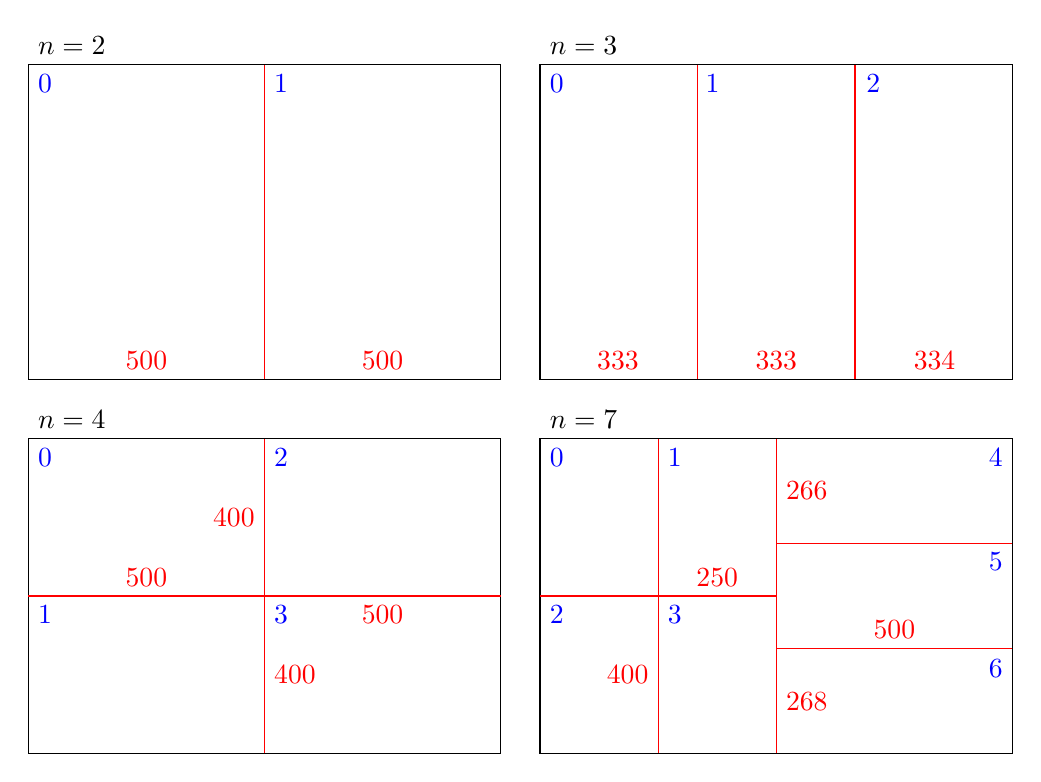
\begin{tikzpicture}[scale=.5]
% 1st rectangle
\draw (0,9.5) --
      (12,9.5)
        node[pos=.25,above,color=red]{\(500\)}
        node[pos=.75,above,color=red]{\(500\)}
        --
      (12,17.5)--
      (0,17.5)
        node[above right]{\(n = 2\)}
        node[below right,color=blue]{\(0\)}
        node[pos=.5,below right,color=blue]{\(1\)}
        -- cycle;
\draw[color=red] (6,9.5) -- (6,17.5);
% 2nd rectangle
\draw (13,9.5) --
      (25,9.5)
        node[pos=.165,above,color=red]{\(333\)}
        node[pos=.5,above,color=red]{\(333\)}
        node[pos=.835,above,color=red]{\(334\)}
        --
      (25,17.5) --
      (13,17.5)
        node[above right]{\(n = 3\)}
        node[below right,color=blue]{\(0\)}
        node[pos=.67,below right,color=blue]{\(1\)}
        node[pos=.33,below right,color=blue]{\(2\)}
        -- cycle;
\draw[color=red] (17,9.5) -- (17,17.5);
\draw[color=red] (21,9.5) -- (21,17.5);
% 3rd rectangle
\draw (0,0) --
      (12,0) --
      (12,8) --
      (0,8)
        node[above right]{\(n = 4\)}
        node[below right,color=blue]{\(0\)}
        node[pos=.5,below right,color=blue]{\(2\)}
        -- cycle;
\draw[color=red] (6,0) -- (6,8)
                   node[pos=.25,color=red,right]{\(400\)}
                   node[pos=.75,color=red,left]{\(400\)};
\draw[color=red] (0,4) -- (12,4)
                   node[pos=.25,color=red,above]{\(500\)}
                   node[pos=.75,color=red,below]{\(500\)}
                   node[pos=0,below right,color=blue]{\(1\)}
                   node[pos=.5,below right,color=blue]{\(3\)};
% 4th rectangle
\draw (13,0) --
      (25,0) --
      (25,8)
        node[below left,color=blue]{\(4\)}
        node[pos=.67,below left,color=blue]{\(5\)}
        node[pos=.33,below left,color=blue]{\(6\)}
        --
      (13,8)
        node[above right]{\(n = 7\)}
        node[below right,color=blue]{\(0\)}
        node[pos=.75,below right,color=blue]{\(1\)}
        -- cycle;
% Vertical
\draw[color=red] (19,0) -- (19,8)
                   node[pos=.165,right]{\(268\)}
                   node[pos=.835,right]{\(266\)};
\draw[color=red] (16,0) -- (16,8)
                   node[pos=.25,left]{\(400\)};
% Horizontal
\draw[color=red] (13,4) -- (19,4)
                   node[pos=.75,above]{\(250\)}
                   node[pos=0,below right,color=blue]{\(2\)}
                   node[pos=.5,below right,color=blue]{\(3\)};
\draw[color=red] (19,2.66) -- (25,2.66)
                   node[pos=.5,above]{\(500\)};
\draw[color=red] (19,5.33) -- (25,5.33);
\end{tikzpicture}
\caption{Aufteilung der Welt für \(n \in \{2,3,4,7\}\), Weltgröße: \(800\) $\times$ \(1000\)}
\label{fig:splitting-of-world}
\end{figure}


\subsubsection{Zusätzliche Performance durch Threads}
Trotzdem wird alleine durch MPI unter Umständen noch nicht die gesamte verfügbare Rechenkraft eines einzelnen Rechners ausgenutzt. Mittels MPI bekommt jeder Node nur einen einzelnen Prozess zugewiesen, unabhängig von der verfügbaren Anzahl Kernen. Somit wäre es von Vorteil diese noch zusätzlich mittels Threads für mehr Rechenleistung auszunutzen. Die Threads werden indessen jedoch nur zur Unterstützung in rechenintensiven Abschnitten der Simulation dienen. Es soll somit nicht die Teilwelt in weitere kleinere Welten aufgebrochen werden, welche dann jeweils von einem Thread verwaltet wird. Hierfür würde eine zusätzliche Kommunikation nötig, die abseits von MPI zusätzlich geschehen müsste, und nicht zwingend notwendig wäre, da viele Abschnitte nicht rechenlastig sind. Konkret wird für die Umsetzung der Threads OpenMP verwendet.


% Klassen
% Aufbau der Serialisierung
% Rendering erklären ->
\section{Dokumentation der Implementierung}
\label{sec:documentation}
Im folgenden Teil wird nun die konkrete Implementierung der Lösungswege aus Sektion \ref{sec:lösungsfindung} detailliert beschrieben und erläutert. Diesbezüglich soll vor allem klargestellt werden, wie genau die Lösungen umgesetzt wurden, sowie die konkreten Gründe für die jeweiligen Ansätze herausgearbeitet werden.

\subsection{Allgemeine Struktur}

Bevor im Detail auf die einzelnen Funktionalitäten eingegangen wird, soll zunächst eine Übersicht über den allgemeinen Aufbau des Programms gegeben werden.
Hierzu sei in Abbildung \ref{fig:class-overview} ein UML-Diagramm mit den wichtigsten Zusammenhängen gegeben. Der Kontrollfluss beginnt in der Datei \emph{Main}, wo \emph{Renderer} und \emph{World} mittels derer \emph{setup()} Methode initialisiert werden, bevor in \emph{createEntities()} die initialen \emph{Entities} der \emph{World} hinzugefügt werden, in \emph{commandLineThread()} der \emph{Thread} für die Nutzereingabe auf der Konsole erstellt wird und schließlich -- abhängig davon, ob gerendert werden soll -- entweder die \emph{normalLoop()} oder die \emph{renderLoop()} ausgeführt wird. Die atomare Zeiteinheit stellt hierbei der \emph{Tick} da, welcher einem Schleifendurchlauf entspricht. Auf Grundlage dieses Kontrollflusses werden nun die im Folgenden beschriebenen Funktionalitäten ausgeführt.



\subsection{Neuronale Netze}
Bereits in der Lösungsfindung wurde die Funktionsweise der neuronalen Netze detailliert erläutert (siehe \ref{subsec:neuronale-netze}). Im Folgenden soll auf die wichtigsten Teile der Implementierung eingegangen werden.

\subsubsection{Berechnung des Verhaltens}

Prinzipiell besitzt jedes \emph{LivingEntity} ein \emph{Brain} als Attribut, welches die komplette Entscheidungsfindung implementiert. Die Ausgabe des neuronalen Netzes wird hierbei mittels Matrixoperationen der Klasse \emph{Matrix} berechnet. Sei $y^{(i)}$ hierbei der Zeilenvektor mit dem Ergebnis der letzten Ebene $i$ mit $n$ Neuronen, wobei $y^{(0)}$ direkt die Eingabe und $y^{(\text{numLayers}-1)}$ die Ausgabe eines kompletten Netzes mit numLayers Ebenen (inklusive Ein- und Ausgabe) und $i \in [0, \text{numLayers}-2]$ bezeichnet. Sei $w^{(i)}_{a,c}$ das Gewicht für das Neuron $y_a^{(i)}$ aus der Ebene $i$ als Eingabe für $y_c^{(i+1)}$ aus der Ebene $i+1$ und $b_c^{(i)}$ die zu addierende Konstante für $y_c^{(i+1)}$. Dann ergeben sich die Werte der Neuronen der nächsten Ebene $i+1$ mit $m$ Neuronen durch:

\[
\begin{bmatrix}
    y_0^{(i+1)} & \dots & y_m^{(i+1)}
\end{bmatrix} =
\tanh{ \left(
\begin{bmatrix}
    y_0^{(i)} & \dots & y_n^{(i)}
\end{bmatrix} \cdot
\begin{bmatrix}
    w_{0,0}^{(i)} & \dots & w_{0,m}^{(i)}\\
    \vdots  & \ddots & \vdots\\
    w_{n,0}^{(i)} & \dots & w_{n,m}^{(i)}
\end{bmatrix} +
\begin{bmatrix}
    b_0^{(i)} & \dots & b_m^{(i)}
\end{bmatrix}
\right)
}
\]
beziehungsweise kürzer
\[
y^{(i+1)} = \tanh \left( y^{(i)} \cdot w^{(i)} + b^{(i)}\right)
\]
wobei $\tanh$ auf jedes Element des Zeilenvektors einzeln angewendet wird.

\subsubsection{Die Aktivierungsfunktion}

\begin{figure}
    \centering
    \begin{tikzpicture}
        \begin{axis}[
            xlabel=$x$,
            %ylabel={$\tanh (x)$}
            ylabel style = {align=center},
            ylabel={$x$ \ref{pgfplots:x} \\$\tanh (x)$ \ref{pgfplots:tanh}},
            xmin=-3,
            xmax=3,
            ymin=-2,
            ymax=2
        ]
            \addplot[mark=none,color=red] {tanh(x)};
            \label{pgfplots:tanh}
            \addplot[mark=none,color=black!50] {x};
            \label{pgfplots:x}
        \end{axis}
    \end{tikzpicture}
    \caption{Die Aktivierungsfunktion $\tanh$}
    \label{fig:tanh}
\end{figure}

Wie aus der obigen Formel hervorgeht, wird als Aktivierungsfunktion $\tanh$ verwendet. Wie in Abbildung \ref{fig:tanh} zu sehen, lässt dieser Werte zwischen $-1$ und $1$ nahezu unverändert -- wodurch beispielsweise die Winkel gut weitergegeben werden können -- und garantiert gleichzeitig, dass Ausgaben immer in $(-1,1)$ sind, wodurch beispielsweise nur valide Winkel ausgegeben werden können. Es ist auch zu sehen, dass Winkel im Bereich nah bei $1$ respektive $-1$ nicht exakt wiedergegeben werden, was nicht optimal ist, dafür aber gute Differenzierbarkeit bietet und somit das Training erleichtert. In Anbetracht der Vielfalt an verschiedenen Datentype, welche im gleichen neuronalen Netz verarbeitet werden, stellt sich $\tanh$ dennoch als sinnvoll heraus.

\subsubsection{Normalisierung der Werte}

Zu beachten bleibt die Tatsache, dass die Aktivierungsfunktion nicht auf Werte der Eingabeebene angewendet wird. Dennoch sollte sichergestellt werden, dass sich die Werte in $[-1,1]$ befinden, um zu vermeiden dass Gewichte schon aufgrund der Eingaben teils betragsmäßig deutlich kleiner sein müssen. Dies würde nicht nur beim Training schlechtere Ergebnisse liefern, sondern insbesondere auch bei der Entwicklung durch zufällige Mutation, wie sie in dieser Simulation stattfindet. Könnten bestimmte Gewichte nur in einem betragsmäßig deutlich kleineren Bereich sinnvoll sein, da sie zuerst große Werte in einen Bereich zwischen $-1$ und $1$ bringen müssten, so würden sich Mutationen hier viel stärker auswirken. Gegebenenfalls wären die Mutationen nicht feingranular genug, um gute Ergebnisse zu erreichen.

Werte wie Winkel, welche sich bereits in $[-1,1]$ befinden, benötigen hierbei keine weitere Vorverarbeitung. Die Wasseragilität wird von $[0,1]$ linear auf $[-1,1]$ abgebildet, da hier ein Unterschied im Vorzeichen aufgrund des Wechsels im präferierten Terrain bei dem Wert im Mittelpunkt semantisch sinnvoll scheint. Im Gegensatz hierzu wird die Energie mithilfe der maximalen Energie linear auf $[0,1]$ abgebildet, da hier ein Vorzeichenwechsel in der Mitte der Werte semantisch weniger Sinn ergäbe. Analog werden auch die Distanzen mittels der maximalen Sichtweite nur auf positive Werte abgebildet, allerding in $[0,0.8]$. Grund hierfür ist die Tatsache, dass auch die Möglichkeit besteht, etwas nicht im Sichtradius zu finden. In diesem Fall wird eine noch höhere Distanz von $1.0$ eingegeben. Außerdem wird statt dem zugehörigen Winkel die Richtung angegeben, in welche sich das Lebewesen im letzten \emph{Tick} bewegt hat, um möglichst geringen Einfluss auf das Ergebnis auszuwirken. Boolesche Werte werden prinzipiell als $-1$ oder $1$ angegeben, die restlichen Werte benötigen keine nennenswerte Normalisierung.

\subsubsection{Vortrainieren der Netze}
\label{sssec:pretraining}
Wie bereits in der Lösungsfindung erwähnt, werden die neuronalen Netze im Vorhinein auf bestimmte Fälle trainiert. Die Idee ist hierbei, das Verhalten in bestimmten Situationen vorzugeben, ohne jedoch Angaben zu anderen Situationen in den Trainingsdaten zu haben, sodass dennoch bereits zu Beginn unterschiedliches Verhalten besteht, wie in Abbildung \ref{fig:brain-weights} zu sehen. Hierfür wird ein neuronales Netz zufällig initialisiert und mit zufällig generierten Trainingsdaten trainiert, welche die Bedingungen eines bestimmten Szenarios erfüllen. Dieser Prozess wird wiederholt und alle neuronalen Netze werden in eine Datei geschrieben (siehe \ref{sssec:serialisierung-entities}). Beim Generieren der Lebewesen zu Beginn der Simulation wird für jedes unabhängig ein zufälliges Netz aus dieser Datei gewählt. Hierbei können insbesondere neuronale Netze auch mehrfach oder gar nicht vergeben werden.

\begin{figure}[H]
    \centering
    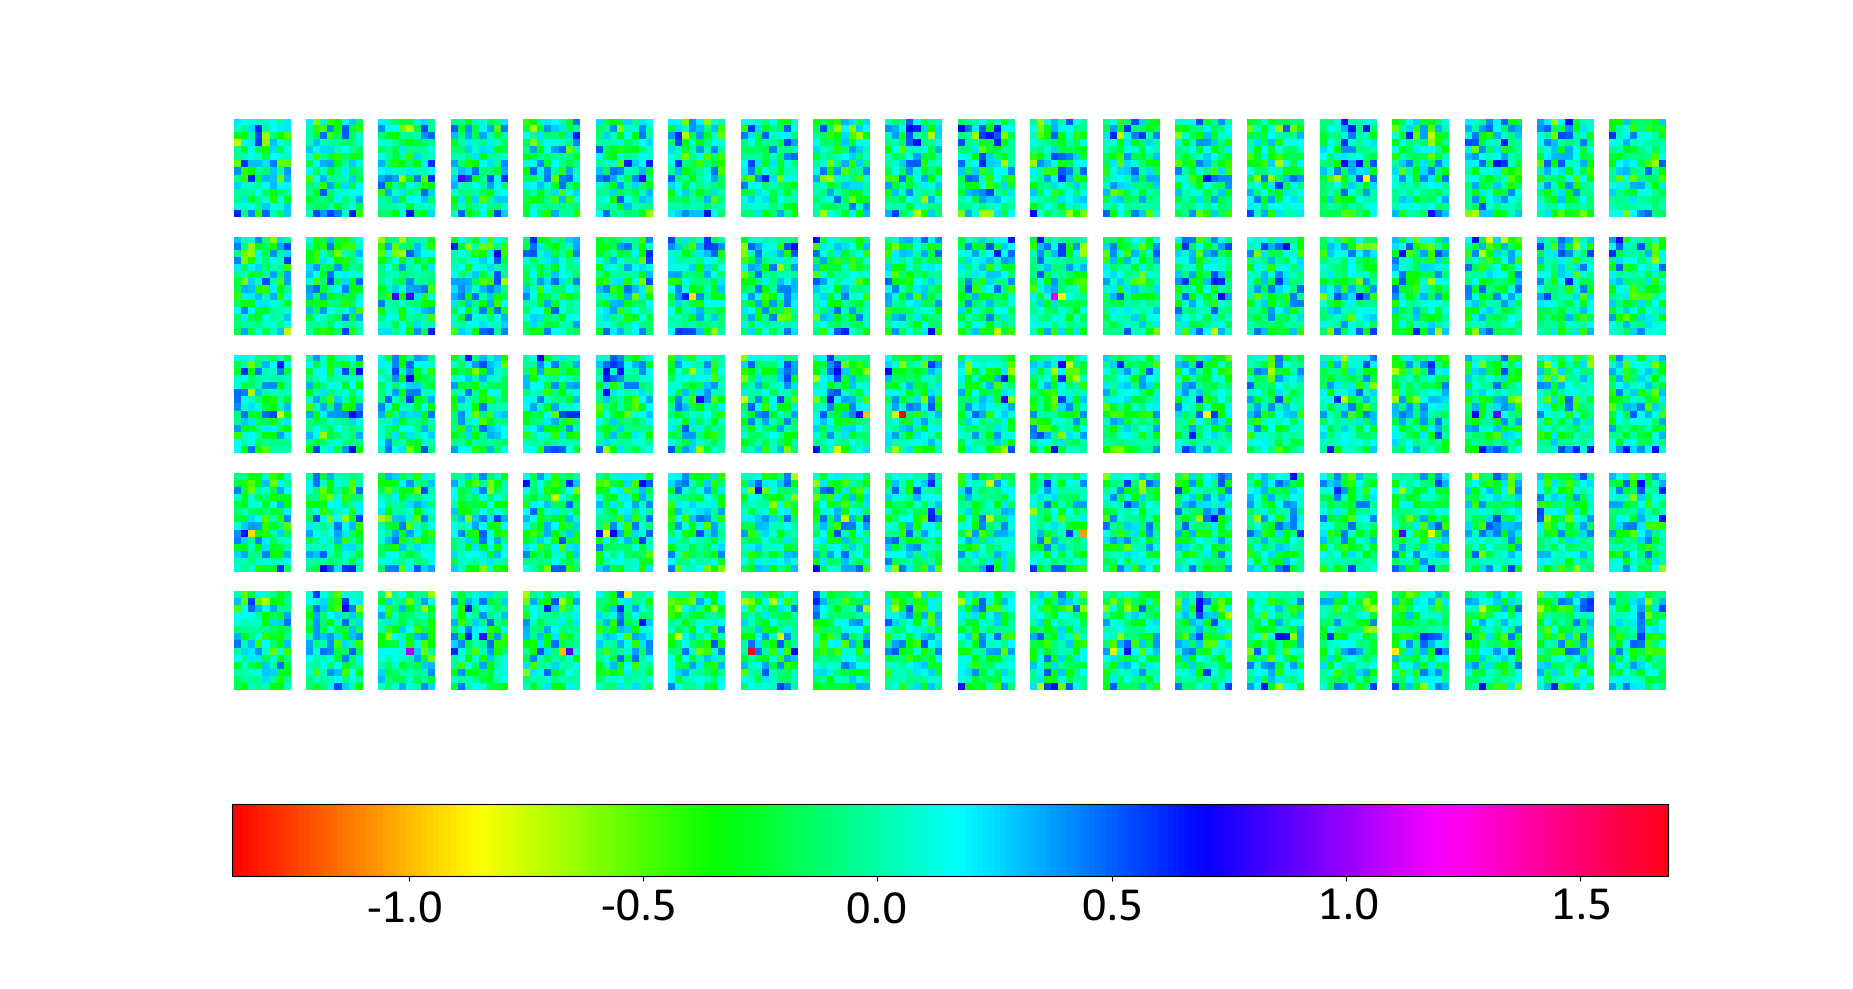
\includegraphics[width=\textwidth]{res/brainsWL0.png}
    \caption{Gewichtungen der vortrainierten neuronalen Netze in der ersten Ebene}
    \label{fig:brain-weights}
\end{figure}

Das konkrete Szenario, welches trainiert wird, ist der Fall, in welchem sich kein anderes \emph{Entity} außer einem \emph{FoodEntity} im Sichtradius befindet, das Entity sich außerhalb der Gefahrenzone am Rand der Welt befindet und sich in Richtung des präferierten Terrains bewegt. In diesem Fall soll sich das Lebewesen so schnell wie möglich zu diesem \emph{FoodEntity} begeben. Angriff und Teilen werden zufällig gesetzt. Zwar würde weder Angriff noch Teilen Sinn ergeben, da sich kein anderes \emph{LivingEntity} in der Nähe befindet, allerdings wird so das sogenannte \emph{overfitting} verhindert. Würden beide Werte auf $-1$ gesetzt, so würden die neuronalen Netze darauf trainiert, in jedem Fall $-1$ auszugeben, da es keine Fälle gibt, in welchen sie auf etwas anderes trainiert werden.

Da das Training ohnehin in einem separaten Programm im Vorhinein erfolgt, wurde hierfür \emph{Python} in Kombination mit den bereits hochgradig optimierten Bibliotheken \emph{Tensorflow} und \emph{Keras} verwendet. Insbesondere benötigt das Vortrainieren abhängig von der gewünschten Anzahl der "`Gehirne"' Zeit im Stundenbereich, was neben der signifikant einfacheren Implementierung des Trainings für diesen Ansatz spricht.

\subsection{Message Passing Interface (MPI)}
\label{subsec:mpi}
Um die Simulation bei gleichbleibenden Startbedingungen performanter und damit auch schneller zu machen, wird dafür zum größten Teil MPI verwendet. Hierfür soll die gesamte Welt in kleinere, disjunkte Teilwelten aufgeteilt werden. Alle Teilwelten werden dann auf eigenständige Prozesse aufgeteilt, welche mittels MPI miteinander kommunizieren können. Auf diese Weise wird es möglich, die Simulation auf beliebig viele Computer in einem Cluster aufzuteilen. Diese müssen in Folge nur noch einen kleineren Teil der Welt eigenständig berechnen. Als Ergebnis soll die Simulation mit steigender Anzahl von Prozessen -- und somit kleineren Teilwelten -- insgesamt performanter werden.

Um im Folgenden die Teilwelten nicht mit den Welten von MPI zu verwechseln, werden diese nun als \emph{Nodes} bezeichnet. Diese sind gleichzusetzen mit den gleichnamigen Nodes in MPI.
Da pro Rechner im Cluster nur ein Prozess läuft, ist die Bezeichnung hierfür legitim. In der Simulation ist die statische Klasse \emph{World} für die Verwaltung der Welten und damit auch die grundlegende MPI Kommunikation zuständig.


\subsubsection{Serialisierung von Entities}
\label{sssec:serialisierung-entities}
Da MPI das Versenden von allgemeinen Objekten zwischen Nodes nicht unterstützt, muss eine andere Möglichkeit zum Versenden der Entities über MPI gefunden werden. Um dies so platzsparend und effizient wie möglich zu gestalten, werden alle benötigten Attributwerte hintereinander in einen Puffer geschrieben, mit Hilfe des Datentyps \emph{MPI\_BYTE} versendet und anschließend in der gleichen Reihenfolge wieder ausgelesen.

Hierfür implementieren beide Klassen \emph{LivingEntity} und \emph{FoodEntity} die Methoden \emph{minimalSerializedSize()} und \emph{minimalSerialize(void*\&)} für das Versenden an Knoten, in deren Pufferbereich sich das Entity befindet, sowie \emph{fullSerializedSize()} und \emph{fullSerialize(void*\&)} für den tatsächlichen Wechsel zwischen Knoten. Während bei Food-Entities kein Unterschied zwischen den Beiden besteht, muss bei Living-Entities das Gehirn -- welches einen Großteil der Datenmenge ausmacht -- nur bei einem tatsächlichen Wechsel gesendet werden, da die Handlungen immer nur auf einem Knoten berechnet werden. Der Versand sämtlicher anderer Attribute ist aufgrund der Bestimmung der Ähnlichkeit zweier Entities immer notwendig.
Auch das \emph{Brain} hat entsprechende Methoden, welche im \emph{LivingEntity} verwendet werden. Das Gegenstück zur Serialisierung bildet jeweils ein entsprechender Konstruktor, welcher mittels eines Pointers das Objekt rekonstruiert.

Zum Versenden wird zuerst durch Summieren der \emph{serializedSize()} die Größe des benötigten Puffers in Bytes ermittelt. Anschließend wird entsprechend Speicher allokiert und auf jedes benötigte Objekt \emph{serialize()} aufgerufen. Der entstandene Puffer wird mittels MPI versendet und mittels der Konstruktoren eingelesen. Sowohl die \emph{serialize()} Methode als auch die Konstruktoren erhöhen hierbei den Pointer automatisch, sodass sie auf das nächste freie beziehungsweise zu lesenden Byte zeigen.
Konkret werden bei der Serialisierung die Bytes hintereinander in den Speicher gelegt, wie in Abbildung \ref{fig:serialization-format} verdeutlicht.

Die Datei brains.dat macht sich die vorhandenen Methoden zu Nutze und verwendet das gleiche Format zur Speicherung der Gehirne.

\begin{figure}
	\centering
	\begin{subfigure}{\linewidth}
    	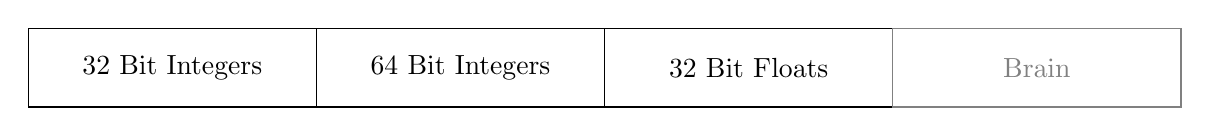
\begin{tikzpicture}[x=1.22cm,y=1cm]
    	\draw (0,0) rectangle (3,1) node[pos=.5] {32 Bit Integers};
    	\draw (3,0) rectangle (6,1) node[pos=.5] {64 Bit Integers};
    	\draw (6,0) rectangle (9,1) node[pos=.5] {32 Bit Floats};
    	\draw [draw=black!50, text=black!50] (9,0) rectangle (12,1) node[pos=.5] {Brain};
    	\end{tikzpicture}
	\caption{Datenlayout des \emph{LivingEntity}s}
    \end{subfigure}\par\medskip
    \begin{subfigure}{\linewidth}
    	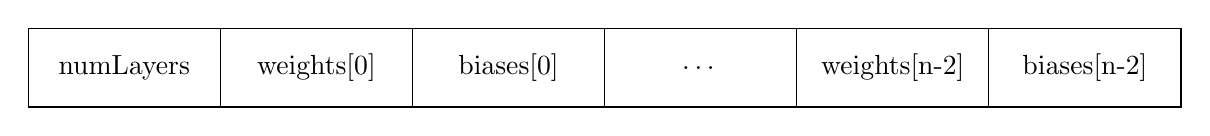
\begin{tikzpicture}[x=1.22cm,y=1cm]
        \draw (0,0) rectangle (2,1) node[pos=.5] {numLayers};
        \draw (2,0) rectangle (4,1) node[pos=.5] {weights[0]};
        \draw (4,0) rectangle (6,1) node[pos=.5] {biases[0]};
        \draw (6,0) rectangle (8,1) node[pos=.5] {\dots};
        \draw (8,0) rectangle (10,1) node[pos=.5] {weights[n-2]};
        \draw (10,0) rectangle (12,1) node[pos=.5] {biases[n-2]};
    	\end{tikzpicture}
	\caption{Datenlayout des \emph{Brain}s}
    \end{subfigure}\par\medskip
    \begin{subfigure}{\linewidth}
    	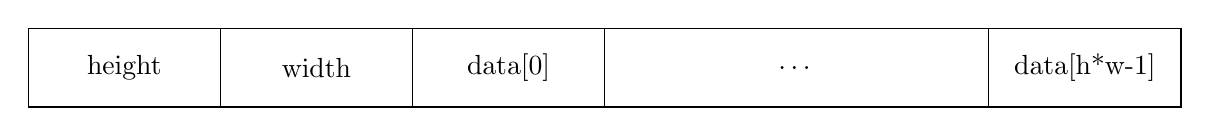
\begin{tikzpicture}[x=1.22cm,y=1cm]
        \draw (0,0) rectangle (2,1) node[pos=.5] {height};
        \draw (2,0) rectangle (4,1) node[pos=.5] {width};
        \draw (4,0) rectangle (6,1) node[pos=.5] {data[0]};
        \draw (6,0) rectangle (10,1) node[pos=.5] {\dots};
        \draw (10,0) rectangle (12,1) node[pos=.5] {data[h*w-1]};
    	\end{tikzpicture}
	\caption{Datenlayout der \emph{Matrix}}
    \end{subfigure}\par\medskip
    \begin{subfigure}{\linewidth}
    	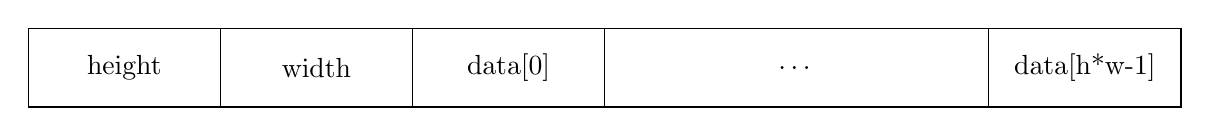
\begin{tikzpicture}[x=1.22cm,y=1cm]
        \draw (0,0) rectangle (2,1) node[pos=.5] {height};
        \draw (2,0) rectangle (4,1) node[pos=.5] {width};
        \draw (4,0) rectangle (6,1) node[pos=.5] {data[0]};
        \draw (6,0) rectangle (10,1) node[pos=.5] {\dots};
        \draw (10,0) rectangle (12,1) node[pos=.5] {data[h*w-1]};
    	\end{tikzpicture}
	\caption{Datenlayout des \emph{Brain}s}
    \end{subfigure}\par\medskip
    \begin{subfigure}{\linewidth}
    	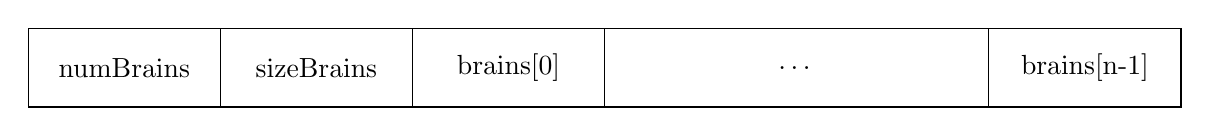
\begin{tikzpicture}[x=1.22cm,y=1cm]
    	\draw (0,0) rectangle (2,1) node[pos=.5] {numBrains};
        \draw (2,0) rectangle (4,1) node[pos=.5] {sizeBrains};
        \draw (4,0) rectangle (6,1) node[pos=.5] {brains[0]};
        \draw (6,0) rectangle (10,1) node[pos=.5] {\dots};
        \draw (10,0) rectangle (12,1) node[pos=.5] {brains[n-1]};
    	\end{tikzpicture}
	\caption{Datenlayout der Datei \emph{brains.dat}}
    \end{subfigure}\par\medskip
	\caption{Datenlayouts bei der Serialisierung}
	\label{fig:serialization-format}
\end{figure}

\subsubsection{Kommunikationssituationen}
Grundsätzlich muss in den folgenden Situationen während der Simulation eine Kommunikation zwischen den einzelnen Nodes stattfinden (als \emph{Root Node} wird im Folgenden immer der Node mit dem Rank 0 bezeichnet):

\begin{enumerate}
\item Austausch der Food- und Living Entities zwischen den Nodes nach jedem Tick.
\item Verteilen der Food- und Living Entities, die vom Root Node zu Beginn generiert werden.
\item Verteilen eines Puffers vom Root Node, welcher für jeden Node einen für 100 Ticks validen Puffer an Food Entities generiert.
\item Broadcasting des aktuellen Status der Simulation (z.B. ob diese pausiert oder beendet wurde, ob gerendert werden soll, etc.) ausgehend vom Root Node.
\end{enumerate}

Alle sonstigen Situationen, wie z.B. das Ticken der Entities und das Rendern der Welt, können die Nodes selbstständig bearbeiten. Im Folgenden sollen nun die Situationen 1. - 4. genauer erläutert und deren Lösung vorgestellt werden.


\subsubsection{Situation 1 -- Austausch der Food- und Living Entities zwischen den Nodes nach jedem Tick}
Dies ist die wohl wichtigste und auch komplizierteste Situation und bildet das Herzstück für die Parallelisierung der Simulation. Es ist die einzige Situation, in der nicht der Root Node als zentraler Knoten für den Austausch dient, sondern die Prozesse sich selbst untereinander koordinieren müssen. Dafür wird jede Node alle Nodes kennen müssen, von denen sie Nachrichten bekommt und an welche sie solche senden muss. Im Weiteren soll dieses Problem nun mit Hilfe des \emph{World Paddings} und den daraus resultierenden \emph{Padding Rechtecken} veranschaulicht und gelöst werden.


\paragraph{World Padding}
Entstanden ist dieser Lösungsansatz unter dem Problem des Renderings der Welt mit mehreren Nodes. Weil jede Node ihre Teilwelt selbst rendern muss, zeigt diese auch nur ihre eigenen Entities an. Problematisch ist es, dass Entities als kleine Kreise (mit ihrer aktuellen Energie darüber) gezeichnet werden. Da dies mehr als nur einen Pixel Platz beansprucht, kann es zu Überlappungen an den Rändern führen. Folglich werden Entities am Rand der Teilwelt abgeschnitten, weil die andere Node das Entity noch nicht bei sich gespeichert hat.

Um dieses Problem zu lösen wird ein allgemeines, festes \emph{World Padding} eingeführt. Dieses gibt den Abstand in Pixeln vom Rand an, in welchem noch Informationen über die Entities sowie die Struktur der Welt gespeichert werden sollen, obwohl dieser Teil nicht mehr zum eigentlich von dieser Node verwalteten Teil gehört. Es ist somit eine Pufferzone, die es ermöglicht, trotzdem Entities vollständig am Rand anzuzeigen, obwohl sich diese sich eigentlich nicht auf der eigenen Teilwelt befinden.


\paragraph{Padding Rechtecke}
Aufgrund der zusätzlichen Pufferzone (World Padding) ergibt sich nun eine Überlappung zwischen den verwalteten Bereichen der Nodes. Folglich muss eine Node, auch wenn sich das Entity noch auf dessen Teilwelt befindet, gegebenenfalls dieses zusätzlich (als Kopie) an andere Nodes in der Umgebung schicken. Damit eine Node nun weiß, auf welchem Stück der eigenen Teilwelt sich eine Pufferzone eines anderen Nodes befindet, werden hierfür \emph{Padding Rechtecke} berechnet.

In diesen speichert sich jede Node den Rank der Node, die eine Überlappung mit ihrer Pufferzone an dieser Stelle hat. Diese Rechtecke können dabei mit einfachen Rechenoperationen berechnet werden, da jede Node die Dimensionen der Teilwelten aller Nodes kennt und das World Padding eine feste Größe ist.

Sei \(R_i = [x_i, y_i, w_i, h_i]\) das Rechteck (Teilwelt mit Pufferzone) der Node mit Rank \(i\) und \(R_e = [x_e, y_e, w_e, h_e]\) das Rechteck (Teilwelt \textsc{ohne} Pufferzone) der Node, für welche die Padding Rechtecke berechnet werden sollen. Damit lässt sich das Padding Rechteck \(P_i = [x, y, w, h]\) (Schnittfläche) für Rank \(i\) wie folgt berechnen \footnote{vgl. \href{https://stackoverflow.com/a/19754915}{https://stackoverflow.com/a/19754915}}:

\[x = max\{x_i, x_e\}, y = max\{y_i, y_e\}\]
\[w = min\{x_i + w_i, x_e + w_e\} - x, h = min\{y_i + h_i, y_e + h_e\} - y\]

Falls \(w > 0 \land h > 0\) ist dies ein valides Rechteck und es existiert wirklich eine Überlappung zwischen der aktuellen Node und der mit Rank \(i\). Diese Berechnung wird nun für alle Ranks durchgeführt und die jeweiligen validen Rechtecke abgespeichert. Da sich die Dimensionen der Welten während der Simulation nie ändern, braucht es diese Berechnung nur einmal vor Beginn der Simulation.


\paragraph{Allgemeine Strategie}
\label{par:allgemeine-strategie}
Die Node, auf welcher sich die Entities befinden (ohne Pufferzone!), ist für alle Entscheidungen zu einem Entity ausschlaggebend. Dies betrifft das Versenden, Hinzufügen und Löschen der Entities. Folglich werden Entities auch nur auf dieser Node getickt. Daher werden Entities, die sich in der Pufferzone befinden, auch nur mit minimal vielen Attributen gespeichert bzw. von der anderen Node versendet (z.B. ohne Brain bei Living-Entities).

Nachdem alle Entities getickt und aktualisiert wurden, werden diese zwischen den Nodes ausgetauscht. Dafür werden jeweils Puffer für Food- und Living-Entities, die gesendet werden sollen, angelegt. Zu jedem Entity wird zusätzlich der Rank gespeichert, an den es gesendet wird. Diese Puffer werden vor und während den Ticks der Entities befüllt.

Der Austausch, ausgehende von einer Node, findet nun in zwei Schritten statt: Zuerst sendet die Node alle zusendenden Entities an die jeweiligen Nodes. Danach wartet sie darauf von anderen Nodes Entities zu empfangen. Hierbei ist es wichtig anzumerken, dass das Senden \emph{non-blocking (MPI\_Isend)} und das Empfangen \emph{blocking (MPI\_Recv)} via MPI stattfindet. Grund hierfür ist, dass bei einem \emph{blocking send} ein Deadlock entstehen würde, weil alle gleichzeitig senden aber niemand empfangen würde. Es würden somit folglich alle Nodes blockieren. Beim \emph{non-blocking send} können alle Nodes, obwohl der Empfänger noch nicht auf Daten wartet, trotzdem die Entities versenden und werden nicht blockiert. Allerdings müssen alle Nodes am Ende darauf warten, dass jede Node ihre Daten empfangen hat, bevor diese weiterrechnen dürfen. Grund hierfür ist, dass der gesendete Puffer erst freigegeben werden darf, sobald der andere Node diesen mit Sicherheit empfangen hat. Dies wird mittels der Funktion \emph{MPI\_Waitall()} umgesetzt, welche erst zurückkehrt, sobald \textsc{alle} Puffer der \emph{MPI\_Isend()}-Aufrufe verschickt wurden.

Der Code zum Versenden der Entities befindet sich in der Methode \emph{sendEntities()} und zum Empfangen in \emph{receiveEntities()} der Klasse \emph{World}.


\paragraph{Senden von Food Entities}
Aufgrund des World Paddings müssen Food-Entities, die sich in mindestens einem Padding Rechteck von einer anderen Node befinden, an die jeweiligen Nodes versendet werden. Da sich Food-Entities nicht bewegen, gestaltet sich der Austausch dieser zwischen den Nodes einfacher als für Living-Entities.

Grundsätzlich müssen Food-Entities nur zu zwei Ereignissen versendet werden: beim Hinzufügen und Löschen. Somit gibt es auch zwei Puffer für zusendende Food Entities. Hierbei werden jeweils die Objekte serialisiert (siehe \ref{sssec:serialisierung-entities}) und dann getrennt versendet. Jede Node versendet somit zwei Nachrichten an die jeweiligen Nodes.

Food-Entities, die hinzugefügt werden sollen, brauchen die Nodes nur noch in ihrer Pufferzone mittels einer Deserialisierung hinzuzufügen. Hingegen müssen die Food-Entities, welche gelöscht werden sollen, zusätzlich anhand ihrer eindeutigen ID aus der Pufferzone entfernt werden. Hierfür wird zuerst das Food-Entity deserialisiert und daraufhin die Pufferzone nach dem Food-Entity mit der selben ID durchsucht. Das daraufhin gefundene Food-Entity wird dann aus der Pufferzone entfernt.


\paragraph{Senden von Living Entities}
Hingegen muss beim Verwalten der Living-Entities in den Pufferzonen mehr Aufwand betrieben werden. Da sich Living-Entities bewegen, werden diese jeweils nach allen Entity Ticks zuerst aus der Pufferzone entfernt. Dies hat den Vorteil, dass Living Entities, welche auf dem ursprünglichem Node entfernet wurden, nicht gesondert versendet werden müssen wie dies bei den Food-Entities der Fall ist.

Somit gibt es nur noch zwei Fälle für das Versenden der Entities: das Entity betritt mindestens ein Padding Rechteck oder es verlässt die aktuelle Node. Bei ersterem kann so fortgefahren werden wie mit den Food Entities. Das Living Entity wird zuerst serialisiert, dann versendet und anschließend in der Pufferzone des jeweiligen Nodes eingefügt.

Letzterer Fall gestaltet sich schwieriger. Hier wird das Living Entity auf der (noch) aktuellen Node gelöscht und \textsc{ausschließlich} an die Node gesendet auf der sich das Entity mit der neuen Position nun befindet. Allerdings muss das Living Entity noch zusätzlich gepuffert werden, da es sich (sehr wahrscheinlich) noch in der Pufferzone der alten Node befindet und die neue Node dieses erst nach dem nächsten Tick an den vorherigen Node sendet. Somit ist garantiert, dass das Entity auch im nächsten Tick von anderen Entities auf der alten Node gesehen werden kann.


\subsubsection{Situation 2 -- Verteilen der Food- und Living Entities, die vom Root Node zu Beginn generiert werden}
\label{subsubsec:mpi-situation-2}
Diese und die folgende Situation sind Ergebnisse der Anforderung, dass die Simulation möglichst \emph{deterministisch} sein soll (unabhängig von der Zahl der Nodes im MPI Cluster, siehe Abs. \ref{subsec:determinismus}). Idee ist, den Root Node zu verwenden um auf diesem alle Entities, die zu Beginn der Simulation hinzugefügt werden, zu generieren. Anschließend verteilt der Root Node daraufhin die Entities an ihre jeweilige Node.

Um dies möglichst performant zu lösen, fügt dieser die zufällig generierten Entities in Buckets ein -- zugehörig zu der jeweiligen Node. Diese werden daraufhin mittels \emph{MPI\_Scatterv()} an alle Nodes verteilt. MPI\_Scatter() alleine reicht hierfür nicht aus, da die Buckets unterschiedliche Größen haben werden. Allerdings gibt es in MPI keine direkte Implementierung, die ein \emph{Array von Listen} verteilen kann. Daher werden die Entities in den Buckets zuerst serialisiert und dann hintereinander (aufsteigend nach den Ranks der Nodes) in einen Puffer geschrieben. Dieser kann daraufhin effizient mittels MPI\_Scatterv() an die Nodes aufgeteilt werden. Nachdem alle Nodes ihren jeweiligen Bucket empfangen haben, brauchen diese den Puffer nur noch zu deserialisieren. Zum Schluss werden dann die Entities von den Nodes letztendlich in die Welt eingefügt. Implementiert ist dieser Teil der MPI Kommunikation in der Funktion \emph{createEntities()} der Datei \emph{Main.cpp}.


\subsubsection{Situation 3 -- Verteilen eines Puffers vom Root Node, welcher für jeden Node einen für hundert Ticks validen Puffer an Food-Entities generiert}
\label{subsubsec:mpi-situation-3}
Das Grundprinzip für das Verteilen ist fast identisch zu dem in der zweiten Situation. Auch in dieser Situation werden vom Root Node die generierten Food-Entities in die jeweiligen Buckets gelegt (ausgehend davon zu welchem Node sie gehören) und daraufhin mittels \emph{MPI\_Scatterv()} an die Nodes verteilt. Allerdings werden die Food-Entities von den Nodes nicht direkt in die Welt hinzugefügt, sondern von jeder in einem Puffer abgelegt. Grund hierfür ist, dass die Food Entities vom Root Node für 100 Ticks \emph{vorgeneriert} werden. Im Folgenden soll das genaue Verfahren nun veranschaulicht werden.


\paragraph{Generieren von Nahrung}
Grundlage hierfür ist die sogenannte \emph{Food Rate}. Diese gibt an, wie viele Food Entities pro Tick auf einer Fläche von 2000 Tiles hinzugefügt werden sollen. Um dies möglichst fein granular einstellen zu können, ist die Food Rate eine Gleitkommazahl. Ihr abgerundeter Wert wird pro Tick hinzugefügt und der restliche Bruch auf eine vordefinierte Anzahl Ticks gleichmäßig aufgeteilt. Somit kann für jeden Tick vorberechnet werden wie viele Food Entities zur gesamten Welt hinzugefügt werden sollen.


\paragraph{Vorgenerieren von Food Entities}
Für das Vorgenerieren ist nun der Root Node zuständig. Dieser simuliert 100 Ticks und generiert bei jedem Tick, anhand der Food Rate, neue Food Entities. Diese werden in die anfangs erwähnten Buckets gelegt. Zusätzlich wird allerdings noch für jedes Food Entity gespeichert, zu welchem Tick das Entity erstellt wurde. Hiermit weiß später jede Node, wann sie dieses zu ihrer Welt hinzufügen muss.


\paragraph{Verteilen der Food-Entities}
Nachdem der Root Node alle Food-Entities vorberechnet hat, werden diese nun mittels des anfangs beschriebenen Vorgehens an die Nodes verteilt. Dafür werden die Entities in den Buckets serialisiert, die Buckets hintereinander in einen Puffer geschrieben und dieser dann verteilt. Allerdings wird noch vor jedes Entity bei der Serialisierung der Tick geschrieben, wann dieses generiert wurde. Anschließend fügt jeder Node die empfangenen Entities (zusammen mit dem jeweiligen Tick) in den eigenen Puffer hinzu, aus welchem später die Food-Entities entnommen werden.

Nun kann jede Node für die nächsten 100 Ticks zu jedem Tick neue Food-Entities aus dem Puffer holen. Da die Food-Entities aufsteigend nach dem Zeitpunkt der Erstellung in die Buckets eingefügt werden und diese Reihenfolge auch bei der (De-)Serialisierung beibehalten wird, ist der Puffer eine FIFO-Queue. Somit braucht jede Node nur das vorderste Element zu überprüfen, ob es hinzugefügt werden muss, und fügt ggf. dieses (und weitere) zur Welt hinzu.

Implementiert ist dies zum größten Teil in der Methode \emph{fillFoodBuffer()} und teilweise in \emph{tick()} -- für die Entnahme der Food-Entities aus dem Puffer -- der Klasse World.


\subsubsection{Situation 4 -- Broadcasting des aktuellen Status der Simulation ausgehend vom Root Node}
Zu Debugging Zwecken und um eine Interaktion mit der Simulation zu ermöglichen, müssen gewisse Flags zwischen den Nodes ausgetauscht werden. Hierdurch sollen alle Nodes den selben Status kennen, um beispielsweise gleichzeitig pausieren oder die Simulation beenden zu können. Daher müssen diese vor jedem \emph{World Tick} an alle Nodes, ausgehend vom Root Node, verteilt werden.

Folgende Flags (Tabelle \ref{table:status-flags}) müssen gesendet werden:

% Tabelle für die Statusflags
\begin{table}[H]
\begin{center}
\begin{tabular}{| l | p{10cm} |}
\hline
Status-Flag & Beschreibung \\
\hline
\hline
Run &
Wird die Simulation in der aktuellen Variante (rendern / nicht rendern) ausgeführt? \\
\hline
Render &
Muss die Simulation aktuell gerendert werden? \\
\hline
Paused &
\textsl{(Render Modus)} Ist die Simulation aktuell pausiert?\\
\hline
% TODO: Bessere Beschreibung finden!!!
SimilarityMode &
\textsl{(Render Modus)} Können Entities miteinander verglichen werden? \\
\hline
Borders &
\textsl{(Render Modus)} Sollen die Grenzen der Nodes angezeigt werden? \\
\hline
Paddings &
\textsl{(Render Modus)} Sollen die Padding Rechtecke angezeigt werden?\\
\hline
Quit &
Ist die Simulation beendet worden? \\
\hline
\end{tabular}
\caption{Status-Flags, welche zwischen den Nodes ausgetauscht werden}
\label{table:status-flags}
\end{center}
\end{table}

Um alle Flags einfach versenden zu können, werden diese in einer 8-Bit Bitmap zusammengefasst und anschließend (nachdem alle Eingaben verarbeitet wurden) an die Nodes verteilt. Hierfür wird die \emph{MPI\_Broadcast()} Funktion der MPI Bibliothek verwendet. Root ist hierfür der Node mit dem Rank 0. Anschließend kann jeder Node mit einfachen logischen Bit-Operationen die einzelnen Flags wieder aus der empfangenen Bitmap herausfiltern und übernehmen.

\subsection{Open Multi-Processing (OpenMP)}
Neben der Parallelisierung durch das Aufteilen der Welt auf die vorhandenen Nodes mittels MPI sollen nun auch noch alle Rechenkerne einer einzelnen Node optimal ausgenutzt werden. Dafür bietet es sich an, die rechenintensiven Teile der Simulation auf Threads aufzuteilen. Besonders geeignet ist hierfür die Simulation des Denkprozesses der Entities, da dieser durch die vielen Matrixmultiplikationen zum einen sehr rechenintensiv ist und zum anderen jedes Entity diese Berechnungen unabhängig von allen anderen durchführen kann.

OpenMP war für die Implementierung die naheliegendste Wahl, da es bereits viele Möglichkeiten bereitstellt, um Schleifen zu parallelisieren, ohne dabei die Threads extra verwalten zu müssen. Durch einen Kommandozeilenparameter (siehe \ref{sssec:exec-params}) kann die Anzahl der Threads einfach angepasst werden um die verwendete Hardware optimal auszunutzen.


\subsection{Determinismus}
\label{subsec:determinismus}
Ein weiteres wichtiges Merkmal der Simulation ist, dass sie unter den gleichen Startbedingungen immer dasselbe Ergebnis liefern soll. Die Simulation soll also möglichst \emph{deterministisch} sein. Dies ist vor allem wichtig, um immer wieder zu einem bestimmten Zeitpunkt in der Simulation zurückkehren zu können. Beispielsweise kann dies interessant werden, wenn man wissen möchte, wie sich eine Art weiterentwickelt, aber die Simulation schon beendet wurde. Oder die Simulation ist zu weit fortgeschritten und die Spezies ist schon ausgestorben, man möchte aber analysieren, wieso diese ausstirbt. Damit all dies möglich wird, muss folglich ein Weg gefunden werden, die Simulation deterministisch zu machen.


\subsubsection{Determinismus ohne MPI}
\label{subsubsec:determinismus-ohne-mpi}
Zu Beginn muss die Simulation erst einmal deterministisch auf einer einzelnen Node sein. Dies ist vor allem wichtig, da später durch MPI die Welt in mehrere kleinere Teilwelten aufgeteilt wird und somit je nach Anzahl Nodes sich unterschiedliche Startbedingungen für die Simulation ergeben. Dieses Problem soll im Abschnitt \ref{subsubsec:determinismus-mit-mpi} behoben werden.

Problematisch für den Determinismus ohne MPI ist folgendes: Entscheidungen der Living-Entities (KI) und Zufallszahlen. Mit dem aktuellen Aufbau des neuronalen Netzes, ist dieses von Haus aus deterministisch. Das heißt, es existieren keine äußeren Einflüsse, welche den Output des Netzes zusätzlich beeinflussen, bis auf die Inputs. Somit muss nur sichergestellt werden, dass sich zu einem bestimmten Tick immer dieselben Umstände für ein Entity ergeben, damit das Netz gleiche Inputs bekommt. Da die Startbedingungen jeweils identisch sind, ist der erste Input automatisch deterministisch. Es muss somit nur jeder einzelne World Tick für sich deterministisch sein.

Hierfür kommen nun die Zufallszahlen ins Spiel. Diese sollen einen zufälligen Startzustand der Welt generieren, eine leichte Mutation im Kind-Entity beim Vermehren verursachen und während der Ausführung neue Food-Entities spawnen. Allerdings sollen diese Zufallszahlen nicht von einem "`True Random Number Generator"', z.B. \emph{/dev/random}, kommen, sondern aus einem Pseudo-Zufallszahlen Generator. Dies hat den Vorteil, dass immer gleiche Folgen unter demselben \emph{Seed} generiert werden, was wichtig für den Determinismus ist. In der Simulation werden diese Pseudo-Zufallszahlen durch ein \emph{LFSR-Register} generiert (siehe dazu Abschnitt \ref{subsubsec:lfsr-register}). Der Seed wird beim Starten der Simulation als Programmargument übergeben.

Weil nun die KI wie auch die Zufallszahlen deterministisch sind, ist auch die gesamte Simulation auf einer Node ohne MPI deterministisch. Dies liegt daran, dass zuerst alle Entities für den Start generiert, danach in allen World Ticks immer zuerst Food-Entities gespawnt und daraufhin alle Entity Ticks (zuerst Food- und dann Living-Entities) ausgeführt werden. Somit werden die Zufallszahlen immer in derselben Reihenfolge generiert und jeder bekommt bei jeder Ausführung unter identischen Startbedingungen den selben Wert zur jeweiligen Zeit zugewiesen.


\subsubsection{Einschub: Linear-Feedback Shift Register (LFSR)}
\label{subsubsec:lfsr-register}
Das LFSR besteht aus einem Register in dem zu Beginn ein Anfangswert (\emph{Seed}) steht. Auf dieses Register kann die Operation \emph{step()} ausgeführt werden. Bei dieser werden an bestimmten Positionen (\emph{Taps}) Bits aus dem Register mit einem XOR verbunden und das Resultat (\emph{Output-Bit}) von links an das Register geschoben. Somit wird das Register jeweils um ein Bit nach rechts geschoben. Sollte man die Taps an den richtigen Positionen wählen, kann man so einen maximalen Zyklus erreichen. Mit diesem können dann \(2^n - 1\) verschiedene Binärzahlen generiert werden, wenn das Register \(n\) Bit groß und der Seed \(\neq 0\) ist. Einzig die 0 kann nie erzeugt werden. Hier wäre das Output-Bit stets 0.

Hieraus kann nun ein Pseudo-Zufallszahlen Generator gebaut werden. Da die Folge der Output-Bits für einen Zyklus pseudozufällig ist, kann aus diesen ganz einfach eine Zufallszahl generiert werden. Dafür werden \(m\) Output-Bits, also \(m\) step() Operationen, nacheinander von links in einen Puffer der Größe \(m\) Bit geschoben. Dieser Puffer kann daraufhin zurückgegeben werden und beinhaltet die Zufallszahl. Ggf. muss diese noch normiert werden, um beispielsweise Zahlen in einem gewählten Bereich zu generieren oder eine Gleitkommazahl zu bekommen.


\subsubsection{Determinismus mit MPI}
\label{subsubsec:determinismus-mit-mpi}
Nachdem die Simulation nun auf einer Node deterministisch ist, muss nun das Problem behoben werden, dass sich durch verschiedene Anzahlen von Nodes, bei gleicher Konfiguration der Simulation, unterschiedliche Startbedingungen ergeben. Die KI ist weiterhin deterministisch, da das \emph{World Padding} mindestens so groß wie das Sichtfeld der Living-Entities ist. Die Living-Entities bekommen also die gleichen Einflüsse, wie wenn die Node die gesamte Welt beinhalten würde. Einziges Problem sind hierbei wieder die Zufallszahlen. Problematisch ist, dass nicht jede Node einen eigenen Generator mit demselben Seed bekommen kann. Hierbei würde jede Node die gleiche Folge erzeugen, aber beispielsweise Entities auf unterschiedlichen Nodes identische Teile der Folge erhalten, welche sie auf einer einzelnen Node ohne MPI nicht bekommen hätten. Somit werden nun alle Stellen angepasst, an denen Zufallszahlen benötigt werden.

Ein Problem ist die Generierung der Start-Entities (Startzustand). Unabhängig von der Anzahl Nodes, sollen immer dieselben unter der gleichen Konfiguration erzeugt werden. Hierfür soll der \emph{Root-Node} alle Entities generieren. Anschließend werden diese dann an alle Nodes verteilt (siehe Abs. \ref{subsubsec:mpi-situation-2}). Dies ist nun deterministisch, da der Root-Node einen eigenen Random-Number Generator bekommt aus dem \textsc{alle} Entities für die gesamte Welt auf einmal generiert werden. Somit hängt dies nur noch von der Konfiguration der Simulation ab, also wie viele Entities zu Beginn erstellt werden sollen, die Größe der Welt und der Seed für den Root-Node.

Auch das Spawnen der Food-Entities soll verbessert werden. Der Root-Node generiert hier ebenfalls wieder die Entities mit seinem eigenen Generator und verteilt die Entities daraufhin ebenfalls auf die einzelnen Nodes (siehe Abs. \ref{subsubsec:mpi-situation-3}). Da auch hier wieder die Erstellung der Food-Entities nur von der Konfiguration (hier Food-Rate, Weltgröße, Seed) abhängt, ist die Anzahl Nodes für den Determinismus irrelevant.

% TODO: Serialisierung ist hier etwas unpassend eingeflossen, vlt. an besserer Stelle erwähnen?
Das dritte Problem ist die Erstellung der Kind-Entities. Dieses Problem wird gelöst, indem jedes Living-Entity einen eigenen Zufallszahlen-Generator bekommt. Dieser soll verwendet werden, um die Mutation im Kind-Entity zu berechnen. Der Seed für den Generator des Kind-Entities kommt vom Eltern-Entity. Durch diesen Prozess generiert ein Living-Entity immer dieselben Kind-Entities unter den gleichen Startbedingungen. Der Seed für die Start-Entities kommt hierbei vom Generator des Root-Nodes. Hieraus lässt sich nun auch erklären, warum ein eigenes LFSR-Register implementiert wurde. Dieses wird benötigt, um bei der Serialisierung der Entities den Register-Wert versenden und daraufhin den Generator daraus auf dem anderen Node rekonstruieren zu können.


\subsection{Berechnung des nächstgelegenen Entity's}
Die Living-Entities benötigen in jedem Tick Informationen darüber, wo genau sich nächstgelegenen Entities (nach verschiedenen Kriterien) befinden. Diese lassen sich trivial finden, indem die gesamte Liste der Food- bzw. Living-Entities durchlaufen und das nächstgelegene Entity zurückgegeben wird. Allerdings hat diese Suche für \(n\) Entities eine worst-case Laufzeit von \(\mathcal{O}(n^2)\), da die Suche für jedes Entity in einem Tick durchgeführt werden muss. Somit sollte eine Möglichkeit gefunden werden die Laufzeit zu verbessern. In der trivialen Suche wird schlichtweg die komplette Liste durchlaufen, um das gesuchte Entity zu finden -- ohne Beachtung weiterer Kriterien. Daher wird für die aktuelle Implementierung eine bessere Struktur verwendet, welche die Lokalität der Entities miteinbezieht.

Hierfür wird die Welt in kleine Teile, hier als \emph{Chunks} bezeichnet, zerteilt. Jeder Chunk stellt hierbei einen \emph{Bucket} dar, in welchem Food- bzw. Living-Entities in getrennten Listen abgelegt werden. Sucht man nun nach dem nächstgelegenen Entity, wird zuerst der Bucket durchsucht, in welchem sich das Entity selbst befindet. Sollte die Suche erfolglos sein, wird nun in konzentrischen Kreisen um den Bucket herum nach dem nächstgelegenen Entity gesucht. Die Suche wird nach derjenigen Ebene abgebrochen, in welcher sich maximal noch Entities befinden können, die das Entity sehen kann. Das Ergebnis wird daraufhin zurückgegeben bzw. ein \emph{Nullpointer}, falls kein nächstgelegenes gefunden werden konnte.

In der Implementierung kann nach dem nächstgelegenen Food-Entity mittels \emph{findNearestFood()} bzw. Living-Entity mittels \emph{findNearestLiving()} gesucht werden. Um die Buckets in konzentrischen Kreisen durchsuchen zu können, wird die Methode \emph{searchBucketsForNearestEntity()} von den beiden vorher erwähnten Methoden verwendet. Die Größe eines Chunks beträgt 100 $\times$ 100 Pixel\(^2\). Es ist noch wichtig anzumerken, dass die Buckets eine "`redundante"' Datenstruktur sind. Alle lebenden Living-Entities wie auch die Food-Entities werden weiterhin in einer Liste abgespeichert, um weiterhin alle Entities auf einmal in den Listen durchlaufen zu können.


\subsection{Generierung des Terrains}
Im Abschnitt \ref{subsec:die-welt} wurde das Terrain eingeführt, welches eine Struktur auf der Welt erzeugt. Dabei wurde erwähnt, dass die Tiles, welche zusammen das Terrain bilden, zufällig, aber trotzdem realistisch, auf der Welt verteilt werden sollen. In diesem Abschnitt wird nun der konkrete Ansatz zur Generierung des Terrains erläutert.

Um eine möglichst realistische Verteilung zu bekommen, welche aber trotzdem dem Betrachter als zufällig erscheint, wird eine sogenannte \emph{Perlin-Simplex-Noise} verwendet. Dies ist eine Funktion \(f: \mathbb{R}^n \to [-1,1] \subset \mathbb{R}\), welche zufällige Werte im Intervall \([-1,1]\) annimmt, je nach gesetztem Seed. Der Vorteil einer Noise (im Gegensatz zu einem Random-Number-Generator) ist, dass die Werte im Kontext zueinander stehen, also nahe beieinander liegen. Mathematisch ausgedrückt ist die Funktion \(f\) stetig. Bevor das Terrain jedoch generiert werden kann, sind noch zwei Punkte zu beachten. In der aktuellen Implementierung der Noise, nimmt diese an allen ganzzahligen Stellen den Funktionswert \(0\) an. Daher wird ein Punkt auf der Welt zuerst mit dem Faktor \(\frac{1}{36}\) moduliert, um zu verhindern, dass für alle Punkte \(f(x) = 0\) gilt. Zusätzlich gibt es noch einen \emph{Zoom-Faktor} \(z \in [0.1,\infty)\), welcher das Terrain vergrößert (\(>1\)) bzw. verkleinert (\(<1\)). Effektiv wird somit die Funktion \(f\) mit \(x' = \frac{1}{36} \cdot z^{-1} \cdot x\) aufgerufen.

Mit Hilfe der Noise und unter Beachtung der oben genannten Punkte, kann nun das Terrain erzeugt werden. Sei hierfür \(x \in \mathbb{R}^2\) der modulierte Wert des ursprünglichen Punktes \(x'\) auf der Welt. Der Funktionswert \(f(x) = y\) bestimmt nun den Typus des Tiles: \(-1 \leq y < -0.4\) (Wasser), \(-0,4 \leq y < -0.2\) (Sand), \(-0.2 \leq y < 0.7\) (Grass) und \(0.7 \leq y \leq 1\) (Stein). Aufgrund der Stetigkeit von \(f\), sind die Tiles nun realistisch (zusammenhängend) verteilt. Abschließend ist noch anzumerken, dass für die Generierung nicht jeder Punkt hergenommen wird. Es existiert hierfür eine \emph{TILE\_SIZE}, welche 8 Pixel groß ist und die Höhe/Breite eines Tiles festlegt. Somit wird nur jeder achte Punkt zur Berechnung verwendet.

Die Perlin-Simplex-Noise ist in der Klasse \emph{SimplexNoise} implementiert. Generiert wird das Terrain in der Methode \emph{generateTerrain()} der Klasse \emph{World}.


% TODO: Rendern & Zeichnen nicht vermischen!!!
\subsection{Renderer}
Der Spezifikation aus Abschnitt \ref{subsec:visualisierung-simulation} zufolge, muss es möglich sein, die Simulation in einem Fenster darzustellen. Hierfür soll ein \emph{Renderer} erstellt werden, welcher dieses Fenster anzeigen und mit dem Inhalt aus der Simulation befüllen kann. Im Folgenden wird daher die Umsetzung des Renderers -- implementiert in der gleichnamigen Klasse -- genauer beschrieben und erläutert.

Um das gesamte Rendering der Simulation durchführen zu können, wird als Grundlage die \emph{Simple-DirectMedia-Layer (SDL)} verwendet. Diese Library stellt ein Interface bereit, mit dem plattformunabhängig GUIs erstellt werden können, wobei hier der Fokus auf grafik-intensiven Anwendungen (z.B. Spiele) liegt. Zusätzlich können Ereignisse verarbeitet werden, wie beispielsweise Tastatur- oder Mauseingaben. Da die Simulation grafik-intensiver ist und in anderen Teilen der Simulation auf Eingaben (siehe \ref{sssec:interact-render}) reagiert werden soll, ist die Verwendung der Library für die Implementierung des Renderers vorteilhaft.


\subsubsection{Fundamentaler Aufbau und Basismethoden}
Da für die Simulation nur ein Fenster pro Prozess benötigt wird, ist die Klasse statisch. Der Renderer speichert und verwaltet daher auch nur ein einziges \emph{SDL\_Window} (Fenster). Auf diesem werden dann alle benötigten Texturen für jeweils ein Bild (Frame) eingezeichnet.

Für die grundlegendsten Funktionalitäten existieren die Methoden \emph{renderRect()}, \emph{renderDot()}, \emph{renderFont()} und \emph{renderImage()}. Mit diesen können die fundamentalen Texturen für die Simulation gerendert werden (Rechtecke, Punkte, Texte und Bilder). Die Pointer zu diesen \emph{SDL\_Texture}'s werden von den Methoden zurückgegeben. Aus diesen werden daraufhin die Texturen für die einzelnen Elemente der Simulation zusammengebaut.  Zum Freigeben der Texturen existieren \emph{cleanupTexture()} und \emph{cleanup()}, wobei letztere die gespeicherten Texturen im Renderer löscht. Zusätzlich muss der Renderer initialisiert und nach der Simulation wieder beendet werden. Dies liegt an der SDL-Library, welche ebenfalls zur Benutzung initialisiert und beendet werden muss. Die Methoden \emph{setup()} und \emph{destroy()} übernehmen diesen Schritt.


\subsubsection{Darstellung der Welt und aller Entities}
Zum Darstellen der gesamten Welt müssen das Terrain (Hintergrund) und die Entities gerendert werden. Hierfür wird der Hintergrund zu Beginn einmalig berechnet (\emph{renderBackground}), da sich dieser nie ändert, und daraufhin in jedes Frame kopiert.
Der Hintergrund wird dafür aus den jeweiligen Tiles der Welt zusammengebaut. Für die Tiles existiert jeweils eine 8x8 Pixel große Textur -- jeweils eine für jeden Typus --, welche aus einem Bild vorgerendert wurde.

Beim Rendern der Entities werden ebenfalls die Texturen in eine Gemeinsame für jedes Frame gerendert (\emph{drawEntities}). Für die Food-Entities wird zu Beginn eine Textur (roter Punkt) berechnet, die von allen in jedem Frame genutzt wird. Beim "`Boarisch Mode"' teilen sich diese jeweils eine "`Brezn"' und "`Bier"' Textur. Dies funktioniert, weil jedes Food-Entity die selbe Größe und Farbe hat. Die Living-Entities werden ebenfalls als farbiger Punkt gerendert. Für sie werden jedoch die berechneten Texturen (zusammen mit der ID des Entities) in einem \emph{Cache} gespeichert. Grund hierfür ist, dass Living-Entities verschiedene Größen und Farben haben und somit jeweils eigene Texturen benötigen. Somit wird für jedes Living-Entity nur einmalig seine Textur gerendert, solange es lebendig ist. Die aktuelle Energie wird in jedem Frame über das Entity gezeichnet. Dafür existieren vorgerenderte Texturen der Ziffern 0-9, aus denen die Energieanzeige zusammengebaut wird.


\subsubsection{Ablauf des Zeichnens eines Frames}
Das Frame wird gezeichnet, nachdem der Tick in der World berechnet wurde. Somit kann der aktuelle Status der Simulation im Fenster nun dargestellt werden. Hierfür wird auf ein anfangs leeres Frame zuerst der Hintergrund und danach auf diesen die Entities-Textur, nachdem diese gerendert wurde, kopiert. Zusätzlich werden noch "`Statuselemente"' über die beiden Texturen in das Frame gemalt. Dies umfasst beispielsweise den MPI-Rank und die aktuelle Frame-Rate (Frames-per-second), die in der vergangenen Sekunde erreicht wurde. Nach diesen Schritten kann das vollständige Frame nun mittels \emph{present()} in das Fenster eingezeichnet und angezeigt werden. Damit die Simulation auf eine maximale Frame-Rate limitiert werden kann, wird danach der Prozess für einige Millisekunden schlafen gelegt. Nach dem nächsten Tick wird der Inhalt des Frames mittels \emph{clear()} wieder gelöscht und der beschrieben Prozess beginnt wieder von vorne. Dieser Prozess ist als Teil der Funktion \emph{renderLoop()} in der Datei \emph{Main.cpp} implementiert.


\subsection{Mögliche Verbesserungen der Implementierung}
Trotz der vielen gelösten Probleme in der Implementierung existieren dennoch ungelöste bzw. unvollständig gelöste Probleme. In diesem Abschnitt sollen daher diese aufgezeigt und mögliche Lösungen dafür dargestellt werden.


\subsubsection{Wechsel der Living-Entities zwischen Nodes}
\label{subsubsec:todo-entity-node-change}
In der momentanen Implementierung werden Living-Entities beim Wechsel auf eine andere Node ausschließlich an diese gesendet. Nodes, die an dieser Stelle eine Pufferzone besitzen, können diese Entities somit nicht in ihre eigene Pufferzone einfügen. Schwierig ist hierbei, dass unter Umständen ein Entitiy an eine Position auf dem anderen Node läuft, bei der ein Node eine Pufferzone hat, welche jedoch nicht auf der aktuellen Node zusätzlich eine Überlappung hat. Die Node, die das Entity verschickt, kennt somit diese Node nicht. Daher kann in der aktuellen Implementierung dieses Entity nicht direkt in diese Pufferzone gesendet werden.

Gelöst werden könnte dies über ein Verfahren in zwei Schritten. Zuerst werden die Entities ganz normal wie in der aktuellen Implementierung verschickt. Im zweiten Schritt schicken dann alle Nodes nochmals die empfangenen Living-Entities (aber nur diejenigen, welche auf diesen übergelaufen sind!) an die Nodes. Da jede Node die jeweiligen Zonen und zugehörigen Nodes kennen, können diese die Entities problemlos weitersenden.


\subsubsection{Simulation unter MPI nicht vollständig deterministisch}
Ein weiteres Problem ist, dass trotz der Implementierung aus \ref{subsubsec:determinismus-mit-mpi} die Simulation unter gleicher Konfiguration, aber unterschiedlicher Anzahl Nodes, immer noch nicht deterministisch ist. Lässt man die Simulation jedoch unter gleicher Konfiguration und gleicher Anzahl Nodes laufen, ist die Simulation weiterhin deterministisch. Ein Grund hierfür ist wahrscheinlich das Problem von \ref{subsubsec:todo-entity-node-change}. Hierbei kann es passieren, dass ein Entity am Rand der Teilwelt steht und somit auch Entities aus der Pufferzone für seine Entscheidungen heranzieht. Wenn jedoch Entities beim Node-Wechsel nicht an alle Pufferzonen gesendet werden, sieht das Entity dieses ggf. nicht. Folglich könnte es sich anders entscheiden und dies wäre somit nicht deterministisch für unterschiedliche Anzahl Nodes im MPI-Cluster.


\subsubsection{Falsche Darstellung der Fenster auf High DPI Displays}
Aktuell werden die Fenster auf Displays mit einer hohen DPI Zahl nicht korrekt angezeigt. Beispielsweise werden auf einem MacBook mit Retina Display die Fenster in der richtigen Größe erstellt, allerdings nur zu einem Viertel mit der Anzeige der Simulation befüllt. Unter Linux kann es wiederum passieren, dass sich Fenster Überlappen und somit die gesamte Simulation nicht auf einmal betrachten werden kann. Allerdings bietet SDL hierfür keine Funktion an, mit der für jedes Betriebssystem der Inhalt richtig skaliert wird. Unter Windows existiert beispielsweise die Funktion \emph{SetProcessDpiAwareness()}, welche in Verbindung mit der Flag \emph{SDL\_WINDOW\_ALLOW\_HIGHDPI} beim Erstellen des SDL\_Window's, dem Betriebssystem mitteilt, dass die Simulation High DPI unterstützt.\footnote{siehe z.B. \href{https://seabird.handmade.network/blogs/p/2460-be_aware_of_high_dpi}{https://seabird.handmade.network/blogs/p/2460-be\_aware\_of\_high\_dpi}} Allerdings müsste der Skalierungsfaktor immer noch manuell abgefragt und beim Rendern mit einbezogen werden.

\subsubsection{Aussagekräftigere Konsolenausgabe}
Zwar ist es momentan möglich, die Simulation vollständig ohne Anzeige auszuführen und dabei grundlegende Informationen wie die Anzahl der Living-Entities und Food-Entities in einer Datei zu speichern, allerdings wäre es unter Umständen wünschenswert, aussagekräftigere Informationen zu einer solchen Simulation anzuzeigen. Basierend auf der genetischen Differenz zwischen verschiedenen Living-Entities, welche bereits zur Unterscheidung zwischen Gegner und angehörigem der selben Spezies verwendet wird, könnten sämtliche Living-Entities einer Spezies zugeordnet werden. Da die Anzahl der Spezies nicht im Vorhinein bekannt ist, wäre hierfür beispielsweise \emph{Mean Shift Clustering} geeignet. Anschließend könnten die durchschnittlichen Attributwerte jeder Spezies ausgegeben werden. Hieraus wäre dann beispielsweise ersichtlich, dass sich eine schwimmende Spezies aus relativ großen und eher langsamen Lebewesen entwickelt hat.

Darüber hinaus könnten einige Situationen wie beim Vortrainieren (siehe Abschnitt \ref{sssec:pretraining}) definiert und die Reaktion eines \emph{LivingEntity}s aus einer Spezies auf diese Situationen ausgewertet werden. Daraus ließe sich beispielsweise schlussfolgern, dass es sich bei der obigen Spezies um Jäger handelt, welche auf entsprechende Situationen mit einem hohen Wert für "`Angriff"' reagieren.

Außerdem wäre es denkbar, mittels der bereits existierenden Serialisierung (siehe \ref{sssec:serialisierung-entities}) sämtliche Daten der Welt zu einem Zeitpunkt zu speichern und wieder zu laden. So könnte eine Simulation über längere Zeit auf mehreren Knoten ausgeführt und im Anschluss daran der aktuelle Zustand auf einem anderen Gerät mit potenziell weniger Rechenleistung aber einer Möglichkeit zur Anzeige angesehen werden.


\section{Ergebnisse}
Nachdem im vorhergehenden Abschnitt auf die Implementierung unserer Anwendung eingegangen wurde, soll nun überprüft werden, inwieweit die Simulation den Prozess der Evolution tatsächlich abbildet und wie sich die Parallelisierung auf die Geschwindigkeit und Skalierbarkeit der Anwendung auswirkt.

\subsection{Simulation der Evolution}
Einige Grundtendenzen der Evolution lassen sich in unserer Simulation bereits erkennen. Das Offensichtlichste ist wohl, dass alle Lebewesen, die nicht zumindest ansatzweise sinnvollen Aktionen ausführen, sehr schnell aussterben. Für die dann noch übrigen Lebewesen gibt es zwei Hauptentwicklungsrichtungen. Entweder sie überleben zwar noch etwas länger, sterben dann aber ebenfalls nach einiger Zeit aus, oder sie setzen sich durch und es entwickelt sich eine Spezies dieser Art von Lebewesen. In Abbildung \ref{fig:ergebnisse-simulation-1} hat sich beispielsweise eine Spezies auf Land (dunkelgrün) und eine im Wasser (hellgrün) gebildet.

Von den Aktionen, die einem Lebewesen zur Verfügung stehen, ist die Fortbewegung zur nächsten Nahrung am besten ausgeprägt. Das ist die logische Konsequenz aus der natürlichen Selektion des vorhergehenden Absatzes, da so die Überlebenschancen eines Lebewesens am meisten verbessert werden. Die weiteren möglichen Aktionen - ein gegnerisches Lebewesen anzugreifen oder mit einem Lebewesen der eigenen Spezies Energie zu teilen - sind weitaus weniger ausgeprägt. Die Möglichkeit zur Teilung der Energie ist noch häufiger zu sehen, meistens direkt nach der Fortpflanzung vom Elternteil zum Kind beziehungsweise andersherum. Ein Kampf zwischen zwei Lebewesen ist auf der anderen Seite sehr selten. Das liegt vermutlich daran, dass zwei feindliche Lebewesen weitaus seltener in der Nähe zueinander sind als zwei der gleichen Spezies und somit eine stark ausgebildete Aggressivität kaum Vorteile bringt.

Sehr auffällig ist auch, dass es keinen Lernprozess eines einzelnen Individuums gibt und auch der Lernprozess durch Fortpflanzung nur sehr eingeschränkt ist. In der Abbildung \ref{fig:ergebnisse-simulation-1} stehen viele der hellgrünen Lebewesen am Rand des Wassers und versuchen, zu der nächsten Nahrung am Land zu gelangen. Das ist aber nicht möglich, da bei ihnen das Attribut der Wasseragilität zu ausgeprägt ist und sie sich somit nur im Wasser fortbewegen können. Durch den fehlenden Lernprozess stehen sie somit solange an der gleichen Stelle, bis sie entweder sterben oder die Verteilung der Nahrung sich zufällig so ändert, dass eine Nahrung im Wasser wieder am nächsten ist.

Über längere Zeiträume hinweg lässt sich zudem beobachten, wie ganze Spezies aussterben beziehungsweise sich verändern. Abbildung \ref{fig:ergebnisse-simulation-2} zeigt die gleiche Simulation wie Abbildung \ref{fig:ergebnisse-simulation-1}, nur zu einem späteren Zeitpunkt. Die hellgrüne Wasserspezies existiert noch, aber die dunkelgrüne Landspezies ist komplett verschwunden und stattdessen existieren nun eine türkise und eine blaue Landspezies. Diese sind durch mehrmalige Mutation bei der Fortpflanzung aus der dunkelgrünen Spezies hervorgegangen und hatten besser abgestimmte Attribute, weshalb sie sich durchgesetzt haben.

\subsection{Skalierung}
Da die Rechendauer für die Simulation mit zunehmender Größe der Welt und Anzahl an Entities schnell zunimmt, ist ein wichtiges Ziel unserer Implementierung, die Simulation durch Parallelisierung schneller ausführen zu können. Um dies zu überprüfen werden mehrere Performanztests durchgeführt, die im nachfolgenden beschrieben sind.

\subsubsection{Testumgebung}
Alle Tests werden auf den HimMUC und MaiMUC Clustern durchgeführt.

Der von uns verwendete Teil des HimMUC Clusters besteht aus 40 ODroid C2 Nodes, jeweils mit einem Amlogic S905 SoC, einer Quadcore ARM Cortex-A53 CPU (1.5 GHz) mit 2GB RAM (912 MHz) und einer 1GBit Ethernetverbindung zwischen den Knoten. Die ODroids werden im 64-Bit Modus betrieben, als Betriebssystem wird Debian 10 mit der Kernel-Version 3.14.79+ eingesetzt. Für das Kompilieren und Ausführen der Anwendung werden GCC 8.3.0, CMake 3.13.4 und OpenMPI 3.0 benutzt.

Der MaiMUC ist ein interaktiver Raspberry Pi Cluster in Form eines Maibaums. Er besteht aus 10 Raspberry Pi 3B+ Nodes, jeweils mit einem Broadcom BCM2837 SoC, einer Quadcore ARM Cortex-A53 CPU (1.2GHz) mit 1GB RAM (900MHz) und einer Broadcom VideoCore IV GPU. Die Knoten sind mit 1Gbit Ethernet verbunden (die tatsächliche Bandbreite ist durch die interne Anbindung über USB aber deutlich geringer) und besitzen jeweils noch einen 3.5" Touchscreen mit einer Auflösung von 800px $\times$ 600px. Die verwendeten Programme sind GCC 6.3.0, CMake 3.7.2, SDL 2.0.5, SDL\_ttf 2.0.14, SDL\_image 2.0.1 und MPICH 3.2. Als Betriebssystem läuft Raspbian 9.4 mit der Kernel-Vesion 4.14.70-v7+.

\subsubsection{Verteilung der Rechenzeit}
\label{sssec:computing-times}
Um den Effekt der Skalierung besser beurteilen zu können muss zuerst ermittelt werden, welche Bereiche des Programms die meiste Rechenzeit benötigen. Dazu wurde auf dem MaiMUC einmal die Anwendung auf dem ganzen Cluster mit jeweils 1.000 Living- und Food-Entities und einmal auf einer einzelnen Node mit einer Weltgröße von 1.000px $\times$ 1.000px und je 200 Living- und Food-Entities ausgeführt. Zudem wurde auf dem HimMUC eine Konfiguration von 10.000px $\times$ 10.000px mit je 20.000 Living- und Food-Entities mit 1 bis 10 Nodes ausgeführt. Die Ergebnisse der Tests sind in Abbildung \ref{fig:computing-time} zu sehen.

Der größte Teil der Anwendung wird im Rendering verbracht. Wenn man das außer Acht lässt, wird die meiste Zeit im \emph{Tick} benötigt, weshalb dieser in nochmals in die zwei Bereiche \emph{Denken} und \emph{MPI} unterteilt wurde. Denken beinhaltet dabei den Denkprozess der Entities, also das Auswerten der Neuronalen Netze inklusive der Berechnung der nächsten Position und MPI enthält die Kommunikation der Nodes untereinander. Bei den Messungen auf dem HimMUC lässt sich gut erkennen, dass mit steigender Anzahl an Nodes die Zeit im Denkprozess sinkt, während die Zeit, die mit MPI-Kommunikation verbracht wird, steigt.

Desweiteren ist zu erkennen, dass bei manchen Anzahlen an Nodes, wie zum Beispiel 5 und 7, die MPI-Kommunikation auffällig viel Zeit benötigt. Der Grund für diese Abweichungen ist die Aufteilung der Welt wie in Abschnitt \ref{sssec:aufteilung-der-welt} beschrieben. Bei manchen Anzahlen an Nodes wird die Welt durch den rekursiven Ansatz nicht optimal aufgeteilt, wodurch größere Paddingbereiche entstehen und somit mehr Kommunikation erfolgen muss.

\begin{figure}[H]
\centering
\begin{minipage}{.4\textwidth}
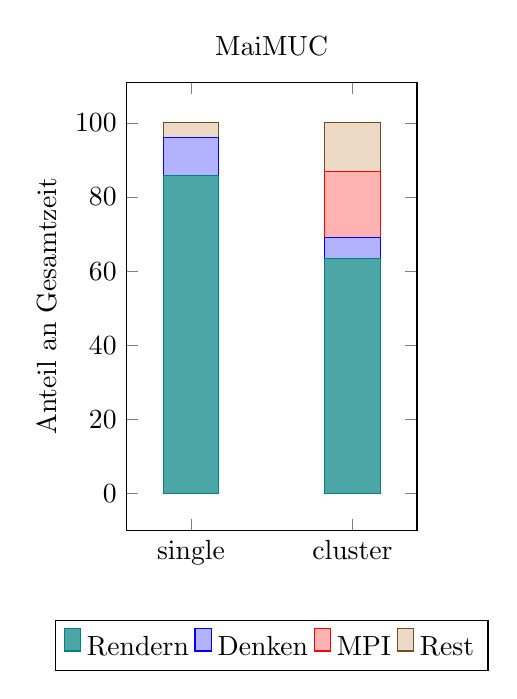
\begin{tikzpicture}
\begin{axis}[
    width=150pt,
    height=\axisdefaultheight,
    ybar stacked,
	bar width=20pt,
    enlarge x limits=0.4,
    legend style={at={(0.5,-0.20)},
      anchor=north,legend columns=-1},
    ylabel={Anteil an Gesamtzeit},
    symbolic x coords={single, cluster},
    xtick=data,
    ymin=-10,
    cycle list shift=-1,
    title={MaiMUC}
    ]
\addplot+[ybar,teal,fill=teal!70!white,mark=none] plot coordinates {(single,85.8) (cluster,63.5)};
\addplot+[ybar] plot coordinates {(single,10.3) (cluster,5.7)};
\addplot+[ybar] plot coordinates {(single,0) (cluster,17.8)};
\addplot+[ybar] plot coordinates {(single,3.9) (cluster,13)};
\legend{\strut Rendern, \strut Denken, \strut MPI, \strut Rest}
,\end{axis}
\end{tikzpicture}
\end{minipage}%
\begin{minipage}{.6\textwidth}
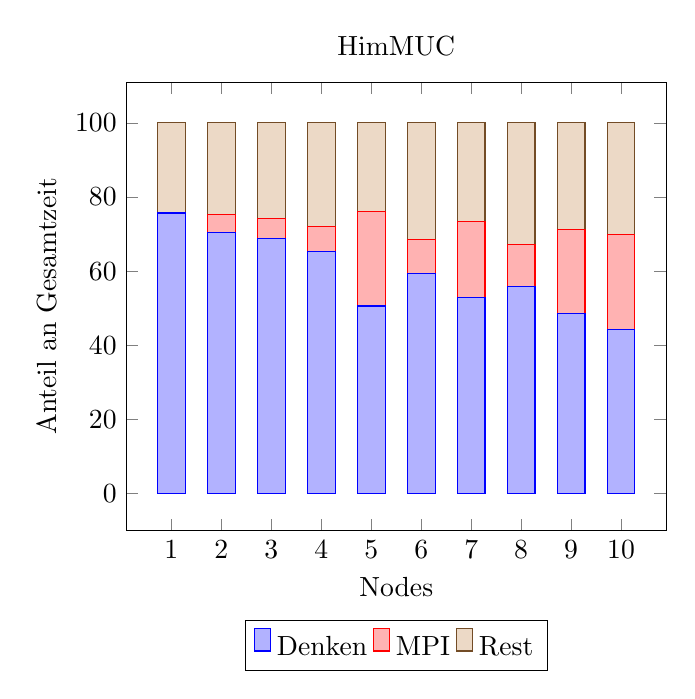
\begin{tikzpicture}
\begin{axis}[
    ybar stacked,
	bar width=10pt,
    enlarge x limits=0.10,
    legend style={at={(0.5,-0.20)},
      anchor=north,legend columns=-1},
    ylabel={Anteil an Gesamtzeit},
    xtick=data,
    xlabel={Nodes},
    ymin=-10,
    title={HimMUC},
    ]

\addplot+[ybar] plot coordinates {(1,75.7) (2,70.4) (3,68.7) (4,65.4) (5,50.6) (6,59.3) (7,52.8) (8,55.8) (9,48.6) (10,44.3)};
\addplot+[ybar] plot coordinates {(1,0) (2,4.9) (3,5.5) (4,6.6) (5,25.4) (6,9.2) (7,20.7) (8,11.4) (9,22.6) (10,25.5)};
\addplot+[ybar] plot coordinates {(1,24.3) (2,24.7) (3,25.8) (4,28) (5,24) (6,31.5) (7,26.5) (8,32.8) (9,28.8) (10,30.2)};
\legend{\strut Denken, \strut MPI, \strut Rest}
\end{axis}
\end{tikzpicture}
\end{minipage}
\caption{Anteil verschiedener Bereiche an der Gesamtrechenzeit}
\label{fig:computing-time}
\end{figure}

\subsubsection{Parallelisierung mit MPI}
Um den Performanzgewinn durch die Verwendung mehrerer Nodes zu testen werden zwei Tests durchgeführt. Im ersten Test wird eine Konfiguration der simulierten Welt festgelegt und dann mit 1 bis 40 Nodes hintereinander ausgeführt. Die simulierte Welt ist 10.000px $\times$ 10.000px groß und initial werden je 20.000 Living- und Food-Entities erzeugt. Beim zweiten Test werden sowohl die Fläche als auch die Anzahl der Entities linear mit der Anzahl der Nodes skaliert. Pro Node wird eine Fläche von 10.000.000px$^{2}$ verwendet sowie je 2.000 Living- und Food-Entities generiert. Ausgehend von der berechneten Fläche wird dann eine quadratische Welt erzeugt, mit den Seitenmaßen abgerundet auf den nächsten ganzzahligen Pixelwert.

Bei beiden Experimenten wird für jede Anzahl an Nodes der gleiche Test je dreimal mit 3.000 Ticks durchgeführt und anschließend der Durchschnittswert genommen. Die dabei erzielten Ergebnisse sind in Abbildungen \ref{fig:himmuc-strong-scaling} und \ref{fig:himmuc-weak-scaling} dargestellt.

\begin{figure}[h]
\centering
\begin{tikzpicture}
\begin{axis}[
xlabel={$Nodes$},
ylabel={$Speedup$}
]
\addplot [blue] table [y expr=920697 / \thisrowno{1}] {data/himmuc-strong-results.dat};
\end{axis}
\end{tikzpicture}
\caption{Skalierung auf dem HimMUC bei einer fixierten Welt mit 10.000px $\times$ 10.000px und je 20.000 Living- und Food-Entities}
\label{fig:himmuc-strong-scaling}
\end{figure}

\begin{figure}
\centering
\begin{minipage}{.5\textwidth}
\centering
\begin{tikzpicture}
\begin{axis}[
width=220pt,
    height=\axisdefaultheight,
xlabel={$Skalierung\;der\;Welt$},
ylabel={$Zeitfaktor$},
legend pos=north west,
]
\addplot [blue] table [y expr=\thisrowno{1}/58807] {data/himmuc-noscaling-results.dat};
\addplot [red] table [y expr=\thisrowno{1}/58527.3] {data/himmuc-weak-results.dat};
\addlegendentry{1 Node}
\addlegendentry{Skalierung der Nodes}
\end{axis}
\end{tikzpicture}
\end{minipage}%
\begin{minipage}{.5\textwidth}
\centering
\begin{tikzpicture}
\begin{axis}[
width=220pt,
    height=\axisdefaultheight,
xlabel={$Skalierung\;der\;Welt$},
legend pos=north west,
]
\addplot [red,mark=*] table [y expr=\thisrowno{1}/58527.3] {data/himmuc-weak-results.dat};
\end{axis}
\end{tikzpicture}
\end{minipage}
\caption{Lineare Skalierung der Fläche und Anzahl an Entities auf dem HimMUC}
\label{fig:himmuc-weak-scaling}
\end{figure}

Bei einer fixierten Weltkonfiguration ist ein Geschwindigkeitsgewinn durch das Hinzufügen von Nodes klar erkennbar. Bis zu etwas über 20 Nodes verläuft der Speedup abgesehen von einigen Schwankungen grundsätzlich linear, danach gibt es bei 24 sowie zwischen 30 und 33 Nodes nochmal einen super-linearen Anstieg, nach denen der Speedup jeweils wieder sub-linear wird.

Wenn die Welt linear skaliert wird, wächst die Ausführungszeit bei gleichbleibender Anzahl an Nodes ebenfalls relativ linear aber circa doppelt so schnell an. Bei einer Skalierung der Welt um den Faktor 40 benötigt eine Node also fast das 80-fache an Rechenzeit. Wenn nun die Anzahl der Nodes ebenfalls linear mitskaliert wird, befindet sich der Zeitfaktor nur noch im Bereich 1 bis 2, schwankt dabei allerdings ziemlich stark. Besonders günstige Anzahlen an Nodes sind 3, 4, 8, 12, 24, 32 und 34, da bei diesen der Zeitfaktor am geringsten ist, während er bei 2, 5, 11, 20 am schlechtesten ausfällt.

Insgesamt skaliert die Anwendung mit zusätzlichen Nodes also sehr gut. Dass der Speedup mit steigender Anzahl an Nodes abflacht war zu erwarten, da ab einem gewissen Punkt jede Node bereits relativ wenige Entities berechnen muss, sodass eine weitere Aufteilung kaum mehr Nutzen hat. Die Skalierung der Welt mit den Nodes lässt keine solchen Tendenzen erkennen, es ist somit zu vermuten, dass auch noch größere Anzahlen an Nodes problemlos möglich wären. Bei beiden Arten der Skalierung ist zu erkennen, dass manche Konfigurationen an Nodes bessere Ergebnisse bewirken als andere. Der Grund dafür wurde bereits im vorhergehenden Abschnitt erläutert.

\subsubsection{Parallelisierung mit OpenMP}
Die zweite Art der Parallelisierung wird mittels OpenMP realisiert. Um dies zu testen, werden zwei Tests auf dem MaiMUC und ein Test auf dem HimMUC durchgeführt. Auf dem MaiMUC wird die Standardkonfiguration (10 Nodes, jede Node berechnet einen Bereich von 800px $\times$ 600px, was der Größe eines Displays entspricht) mit initial je 1.000 Living- und Food-Entities verwendet und einmal mit Rendering und einmal ohne getestet. Auf dem HimMUC wird eine einzelne Node verwendet und die Größe der Welt auf 10.000px $\times$ 10.000px festgelegt, sowie 20.000 Living- und 3.000 Food-Entities erzeugt. Alle Tests werden dann für 3.000 Ticks jeweils dreimal mit ein bis vier Threads ausgeführt und pro Threadanzahl der Durchschnittswert der drei Läufe genommen. Die Ergebnisse der Tests sind in der Abbildung \ref{fig:thread-scaling} zu sehen.

\begin{figure}[h!]
\centering
\begin{tikzpicture}
\begin{axis}[
    xlabel={$Threads$},
    ylabel={$Speedup$},
    xtick={1, 2, 3, 4},
    legend pos=north west,
]
\addplot [blue,mark=*] table [y expr=940218 / \thisrowno{1}] {data/himmuc-threads-results.dat};
\addplot [red,mark=*] table [y expr=16839.7 / \thisrowno{1}] {data/maimuc-threads-results.dat};
\addplot [black,mark=*] table [y expr=98709.3 / \thisrowno{1}] {data/maimuc-threadsrender-results.dat};

\addlegendentry{HimMUC}
\addlegendentry{MaiMUC}
\addlegendentry{MaiMUC (Render)}

\end{axis}
\end{tikzpicture}
\caption{Skalierung mit mehreren Threads bei einer fixierten Welt mit 10.000px $\times$ 10.000px und je 20.000 Living- und Food-Entities}
\label{fig:thread-scaling}
\end{figure}

Auf dem HimMUC ist ein deutlicher Speedup mit mehreren Threads zu erkennen, während er auf dem MaiMUC ohne Rendering für 2 und 3 Threads weitaus geringer ausfällt und bei 4 Threads sogar wieder absinkt. Mit Rendering ist der Speedup kaum existent und wird bei 4 Threads negativ.

Der Grund für den Performanzgewinn auf dem HimMUC ist, dass dort eine bedeutend größere Welt berechnet wird und diese nur auf einem Node ausgeführt wird. Auf dem MaiMUC ist sowohl die Welt bedingt durch die Größe der Displays kleiner und zudem wird sie bereits von 10 Nodes berechnet, wodurch eine einzelne Node nicht mehr viele Entities zu berechnen hat. Mit Rendering wird dieser Speedup dann nochmal inkonsequenter, da das Rendering weitaus mehr Zeit verbraucht als die tatsächlichen Berechnungen (vgl. Abschnitt \ref{sssec:computing-times}). Damit die Verwendung mehrerer Threads also einen Vorteil bringt müssen genug Entities pro Node vorhanden sein, um die einzelnen Rechenkerne auch tatsächlich sinnvoll ausnutzen zu können, da ansonsten der Verwaltungsmehraufwand der Threads überwiegt.

\subsubsection{Vergleich von MPI und OpenMP}
MPI bietet die Möglichkeit, die Anzahl der Prozesse, die pro Node erzeugt werden, zu konfigurieren. Deshalb soll in diesem Test nun evaluiert werden, ob die Parallelisierung einer Node mittels Threads (OpenMP) oder Prozessen (MPI) effektiver ist. Dafür wird auf dem HimMUC die Simulation auf einer Node ausgeführt und einmal ein Prozess und vier Threads, zwei Prozesse und zwei Threads, sowie vier Prozesse und 1 Thread verwendet. Außerdem wird für die gleiche Welt einmal nur die Anzahl der Prozesse und einmal nur die Anzahl an Threads erhöht. Für den Test wurde wieder eine Weltkonfiguration von 10.000px $\times$ 10.000px mit initial je 20.000 Living- Food-Entities benutzt. Wie immer wurde jeder Lauf dreimal ausgeführt und der Durchschnittswert berechnet. Die Ergebnisse sind in Abbildung \ref{fig:threads-vs-processes} dargestellt.

\begin{figure}
\centering
\begin{minipage}{.5\textwidth}
\centering
\begin{tikzpicture}
\begin{axis}[
width=220pt,
    height=\axisdefaultheight,
    xlabel={$Prozesse / Threads$},
    ylabel={$Speedup$},
    xtick={1, 2, 3, 4},
    legend pos=north west
]
\addplot [blue,mark=*] table [y expr=920697 / \thisrowno{1}, restrict x to domain=1:4] {data/himmuc-strong-results.dat};
\addplot [red,mark=*] table [y expr=940218 / \thisrowno{1}] {data/himmuc-threads-results.dat};
\addlegendentry{Prozesse}
\addlegendentry{Threads}
\end{axis}
\end{tikzpicture}
\end{minipage}%
\begin{minipage}{.5\textwidth}
\centering
\begin{tikzpicture}
\begin{axis}[
width=220pt,
    height=\axisdefaultheight,
    xtick=data,
    xticklabels={$1P/4T$, $2P/2T$, $4P/1T$},
    xlabel={$Prozesse / Threads$},
]
\addplot table [x index=0,y expr=336354 / \thisrowno{2}] {data/himmuc-threadsvsprocesses-results.dat};
\end{axis}
\end{tikzpicture}
\end{minipage}
\caption{Vergleich der Skalierung zwischen Prozessen und Threads bei einer fixierten Welt mit 10.000px $\times$ 10.000px und je 20.000 Living- und Food-Entities}
\label{fig:threads-vs-processes}
\end{figure}

Während der Speedup bei der Verwendung von Prozessen linear ist, wird mit Threads nur ein sub-linearer Speedup erreicht. Auch der direkte Vergleich der drei Kombinationen zeigt, dass 4 Prozesse mit je einem Thread um einen Faktor von mehr als 1.3 schneller sind als ein Prozess mit 4 Threads.

Die Verwendung mehrerer MPI-Prozesse ist also eindeutig effektiver im Vergleich zu mehreren Threads. Der Hauptgrund dafür ist, dass mit OpenMP nur ein kleiner Teil der Anwendung parallelisiert wird (der Denkprozess der Entities). Dieser ist zwar ein großer Faktor der Gesamtzeit, aber nicht alles. Der Overhead, der durch die MPI-Kommunikation erzeugt wird, ist also offensichtlich weitaus geringer als der dadurch erreichte Geschwindigkeitsgewinn.

\subsubsection{Zusammenfassung}
Die Messergebnisse haben klar gezeigt, dass die Simulation gut skalierbar ist. Besonders die Skalierung der Welt mit steigender Anzahl an Nodes ist vielversprechend, da dadurch die Grundvoraussetzung geschaffen ist, um große Welten in annehmbarer Zeit berechnen zu können. Ein wichtiger Grund dafür ist sicher auch, dass die Kommunikation direkt zwischen den einzelnen Nodes stattfindet und nicht über einen Master-Node, der bei steigender Nodeanzahl irgendwann ein Engpass werden kann. Mit der aktuellen Implementierung könnte irgendwann höchstens die initiale Generierung der Entities bzw. die Verteilung der Food-Entities problematisch werden, da dies nur auf einem Knoten berechnet wird.

Die Verwendung von Threads hat sich im Vergleich zu Prozessen als nicht sinnvoll herausgestellt. Zwar sparen Threads den Mehraufwand der MPI-Kommunikation ein, da dieser aber bei wenigen Prozessen im Vergleich zur benötigten Rechenzeit für den Denkprozess der Entities relativ gering ausfällt und zudem gut skaliert macht das keinen großen Unterschied. Zumal bei den Threads auch beachtet werden muss, dass hier ebenfalls ein Verwaltungsmehraufwand entsteht.

\section{Verwendung der Simulation}
Die Simulation kann in verschiedenen Versionen kompiliert und mit unterschiedlichen Parametern ausgeführt werden. Die genaue Verwendung soll im Folgenden beschrieben werden.
\subsection{Kompilieren}
Prinzipiell ist zu beachten, dass hier MPI sowie gegebenenfalls SDL2, SDL2 TTF und SDL2 Image benötigt werden.
Zum Kompilieren stehen bereits vorgefertigte Skripte zur Verfügung. Zunächst muss CMake initialisiert werden:
\begin{lstlisting}[language=bash]
  $ ./utils/init.sh <build type> <render>
\end{lstlisting}
Hierbei kann \emph{<render>} entweder \emph{ON} oder \emph{OFF} sein. Ist das Rendern ausgeschaltet, so wird ohne SDL kompiliert. Für den \emph{<build type>} sind gültige Werte \emph{Release}, \emph{Debug} oder \emph{RelWithDebInfo}. \emph{Release} erzeugt optimierten Code und sollte standardmäßig verwendet werden. \emph{Debug} schaltet alle Optimierungen aus und \emph{RelWithDebInfo} optimiert wie \emph{Release}, behält aber die Debugsymbole.
Anschließend kann wie folgt kompiliert werden:
\begin{lstlisting}[language=bash]
  $ ./utils/build.sh
\end{lstlisting}
Alle Kommandos sollten im Projektverzeichnis ausgeführt werden.

\subsection{Ausführen}
Das kompilierte Programm kann auf einem Linuxsystem wie üblich ausgeführt werden. Sollen im Hintergrund Logos angezeigt werden, können diese einfach im Ordner \emph{res/logos} mit dem Namen \emph{<MPI\_Rank>.png} abgelegt werden. Die Bilder werden dann auf dem entsprechenden Knoten angezeigt.
\subsubsection{Parameter}
\label{sssec:exec-params}
Darüber hinaus lässt sich die Simulation mit einer Reihe von Parametern ausführen, um beispielsweise die Größe der Welt, die Anzahl der generierten Entities oder den Seed für die Generierung der Zufallszahlen anzupassen. In Tabelle \ref{table:parameters} im Anhang sind alle möglichen Parameter mit einer kurzen Beschreibung aufgelistet.

\subsubsection{Ausführung auf dem MaiMUC}
\label{sssec:exec-maimuc}
Ein Ziel dieses Praktikums war es, ein Programm zu schreiben, das unter anderem auf dem MaiMUC ausgeführt werden kann. Um die Ausführung in diesem Spezialfall zu vereinfachen, stehen Skripte zur Verfügung. Nach dem Kompilieren auf einem Knoten, findet die Verteilung auf die anderen mit dem Skript \emph{deploy.sh} statt.
\begin{lstlisting}[language=bash]
  $ ./utils/deploy.sh
\end{lstlisting}
Die Ausführung ist im Anschluss wie folgt möglich:
\begin{lstlisting}[language=bash]
  $ ./utils/run.sh ./build/Evolution -m -r <Parameter>
\end{lstlisting}

\subsubsection{Profiling mittels Perf}
Auch zum Profiling mittels \emph{Perf} und der automatischen Erstellung von \emph{Flamegraphs} stehen bereits Skripte zur Verfügung. Auf einem einzelnen Rechner geschieht dies über
\begin{lstlisting}[language=bash]
  $ mpirun -n <Anzahl der Knoten> ./utils/profile-local.sh <Parameter>
\end{lstlisting}
Die generierten \emph{Flamegraphs} befinden sich anschließend im Verzeichnis \emph{perf}.

Auf dem MaiMUC wird - nach entsprechender Vorbereitung (siehe \ref{sssec:exec-maimuc}) - zum Ausführen
\begin{lstlisting}[language=bash]
  $ ./utils/run.sh ./utils/profile-maimuc.sh <Parameter>
\end{lstlisting}
verwendet. Anschließend können mittels
\begin{lstlisting}[language=bash]
  $ ./utils/collect-svg.sh
\end{lstlisting}
die generierten \emph{Flamegraphs} auf dem Knoten \emph{mai02} gesammelt werden.

Um Perf auf dem HimMUC zu verwenden, kann die Ausführung mittels
\begin{lstlisting}[language=bash]
  $ srun -N <Anzahl der Knoten> ./utils/profile-himmuc.sh <Parameter>
\end{lstlisting}
erfolgen.

\subsection{Interaktion}
Auch während der Ausführung kann mit der Simulation sowohl über die Konsole als auch gegebenenfalls durch das angezeigt Fenster interagiert werden. Die Möglichkeiten hierzu sollen im Folgenden aufgezeigt werden.
\subsubsection{über das Fenster}
\label{sssec:interact-render}
Wird die Simulation angezeigt, so kann durch Mausklick sowie einige Tasten auf der Tastatur interagiert werden, um beispielsweise Nahrung zu erzeugen, die Simulation anzuhalten oder die Grenzen der einzelnen MPI-Nodes visuell einzublenden. Anzumerken ist hierbei, dass Mausklicks auf allen Knoten funktionieren, während Interaktion über die Tastatur nur auf dem Knoten mit \emph{MPI\_RANK} 0 möglich ist. Laufen mehrere Knoten auf einem Gerät, so muss der Fokus auf dem Fenster des entsprechenden Knotens liegen. Eine vollständige Beschreibung aller möglichen Aktionen ist in Tabelle \ref{table:interact-window} im Anhang aufgelistet.

\subsubsection{über die Konsole}
\label{sssec:interact-console}
Sämtliche oben genannten Tasten können auch über die Konsole eingegeben werden. Dies kann nützlich sein, wenn - wie beispielsweise am MaiMUC - keine Tastatur direkt an die ausführenden Geräte angeschlossen ist oder die Simulation ohne Anzeige ausgeführt wird. Zu beachten ist hierbei, dass, solange die Anzeige deaktiviert ist, nur die Kommandos \textbf{Q} und gegebenenfalls \textbf{R} gültig sind.

\textbf{R} ist hierbei ein spezielles Konsolenkommando, welches das Rendern wieder aktiviert, sofern es momentan deaktiviert ist und das Programm im Render-Modus kompiliert wurde.

\subsection{Erklärung der Anzeige}
Nach erfolgreicher Ausführung erscheint ein Bild wie in Abbildung [Link einfügen]. Anzumerken ist hier, dass zur besseren Übersichtlichkeit auf der Abbildung bereits in Rot die Grenzen zwischen MPI Knoten angezeigt werden (siehe \ref{sssec:interact-render}).

Auf den ersten Blick stechen bereits unterschiedlich große, farbige Punkte ins Auge, welche sich über die Welt bewegen. Diese stellen die Lebewesen und somit den Kern der Simulation da. Über ihnen sind weiße Zahlen zu sehen. Hierbei handelt es sich um die Energie der Lebewesen. Erreicht sie den Wert Null, so verschwindet das Lebewesen.

Neue Energie können Lebewesen unter anderem erlange, indem sie Nahrung zu sich nehmen. Die unbeweglichen, roten Punkte, welche über die Welt verteilt sind, stellen diese Nahrung da. Werden sie gefressen, so verschwinden sie von der Welt.

Die farbigen Zonen im Hintergrund stellen die Welt da. Sie besteht aus Wasser, Sand, Grass und Stein. Lebewesen können von Gegnern nicht gesehen werden, wenn sie auf einem Untergrund ähnlicher Farbe sind. Außerdem besitzt jedes Lebewesen ein Attribut, welches darüber entscheidet, wie schnell es sich im Wasser bewegen kann. Entsprechend langsamer ist es auf dem Land, also Sand, Grass und Stein.

Die weiße Zahl rechts oben auf den Knoten zeigt die \emph{FPS} an, also wie viele Bilder aktuell pro Sekunde erzeugt werden. Links oben steht der \emph{MPI\_RANK} des Knotens.


\section{Zusammenfassung}
Abschließend kann festgestellt werden, dass die Simulation trotz der hohen Abstraktion schon viele Ähnlichkeiten zur realen Welt sichtbar macht. Vor allem hat sich gezeigt, dass sich viele Spezies entwickeln, welche unterschiedliche Merkmale und Attribute besitzen und sich beispielsweise mehr auf Land als auf Wasser bewegen. Somit existiert auch aktuell schon eine durchaus realitätsnahe Evolution. Andererseits ist die Evolution trotzdem noch stark limitiert, da die neuronalen Netze nicht sehr komplex aufgebaut sind und nur aus wenigen Attributen bestehen, damit diese besser konvergieren.

Auch bei der Parallelisierung hat sich verdeutlicht, dass durch diese ein großer Performanzgewinn bei der Ausführung verzeichnet werden kann. Hierbei darf jedoch nicht außer Acht gelassen werden, dass die Parallelisierung in der konkreten Implementierung nicht leicht umzusetzen war. Durch die geforderten Bedingungen an die Simulation, wie die Bewegung der Entities und deren Interaktion, mussten mehrere Mechanismen eingeführt werden, um den Mehraufwand der Kommunikation möglichst gering zu halten.

Insgesamt lässt sich daher der Schluss ziehen, dass das Ziel der Simulation, eine möglichst realistische Evolution zu erschaffen, welche zusätzlich parallel auf mehreren Rechner verteilt berechnet werden kann, auf jeden Fall erreicht wurde.

\newpage
\section{Anhang}
\begin{figure} [h]
    \centering
    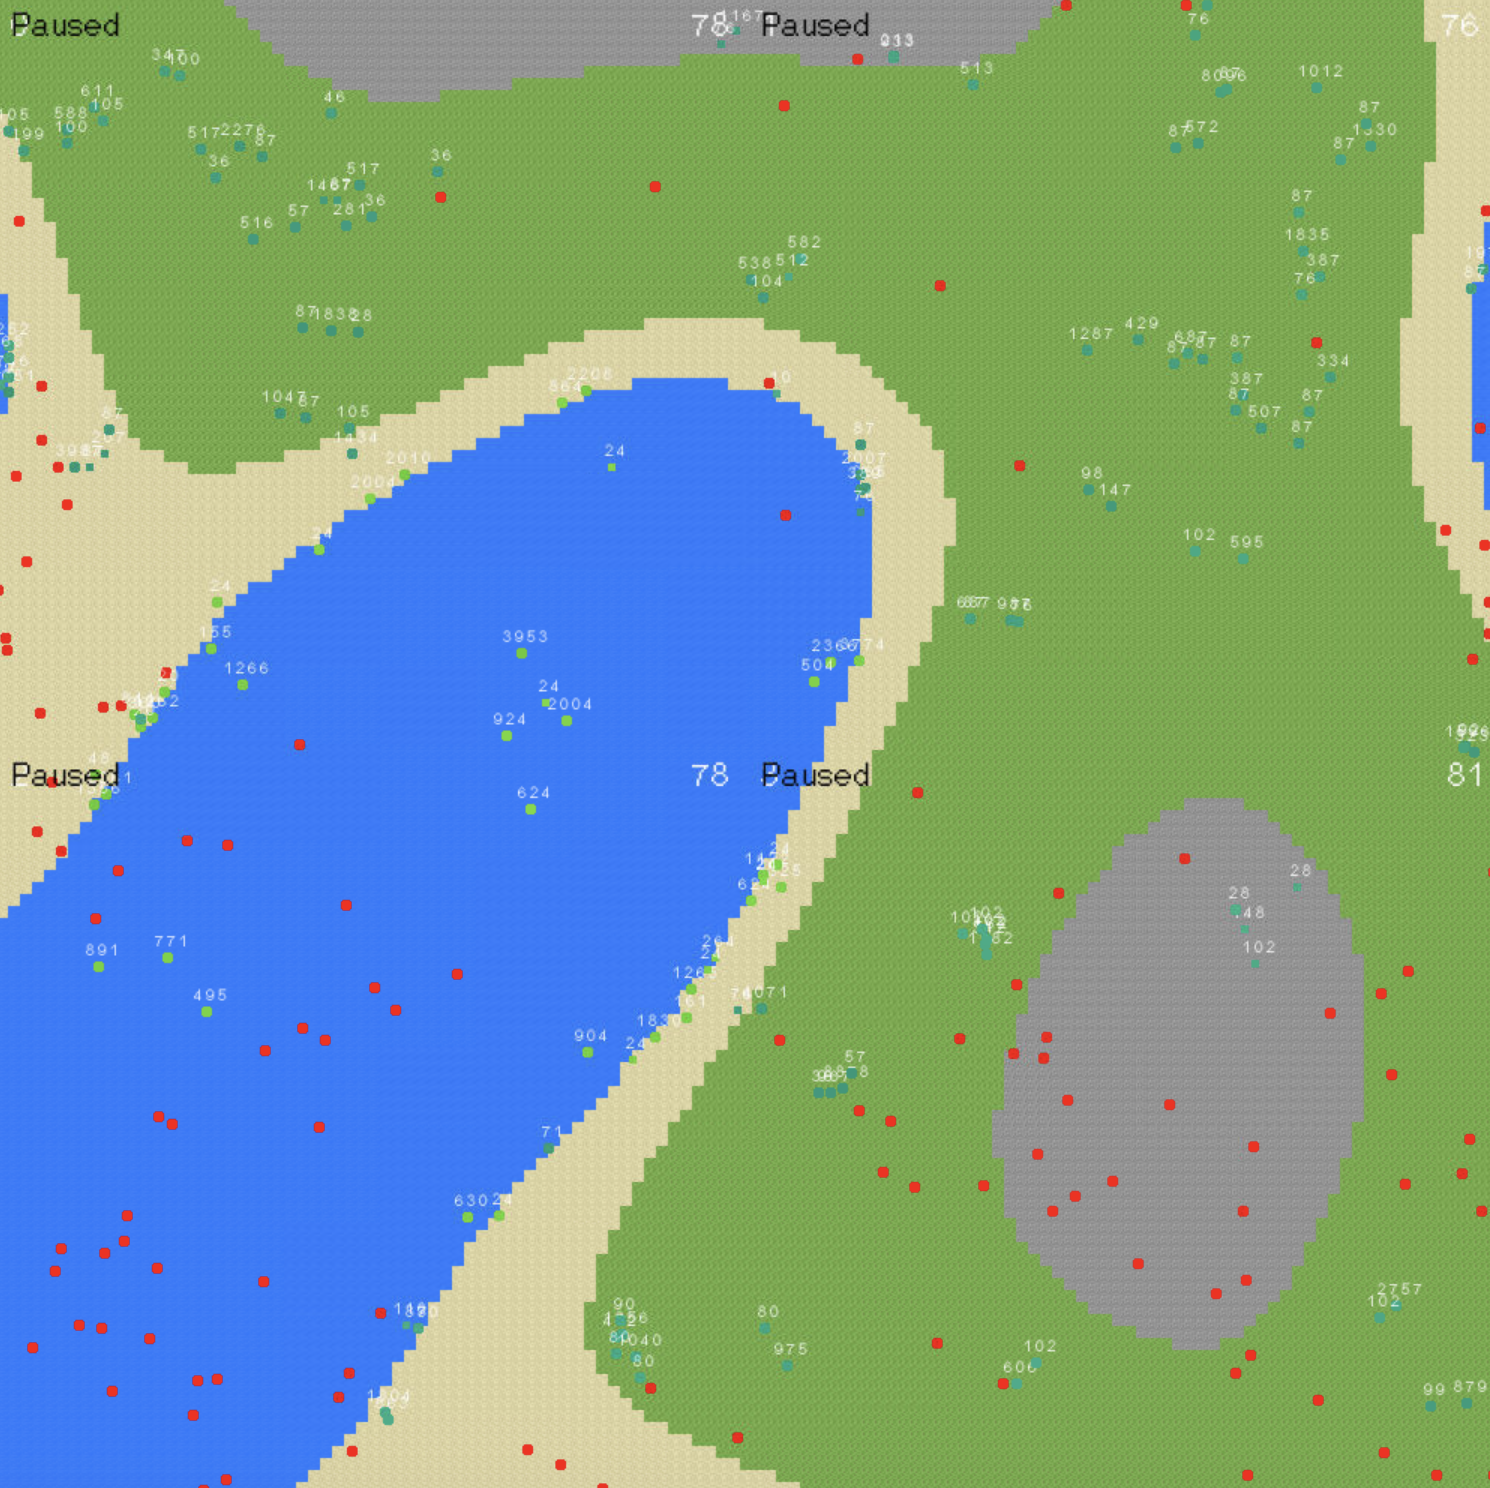
\includegraphics[width=\textwidth]{res/ergebnisse-simulation-1.png}
    \caption{Beispielhafter Ausschnitt der Simulation (1)}
    \label{fig:ergebnisse-simulation-1}
\end{figure}

\begin{figure}
    \centering
    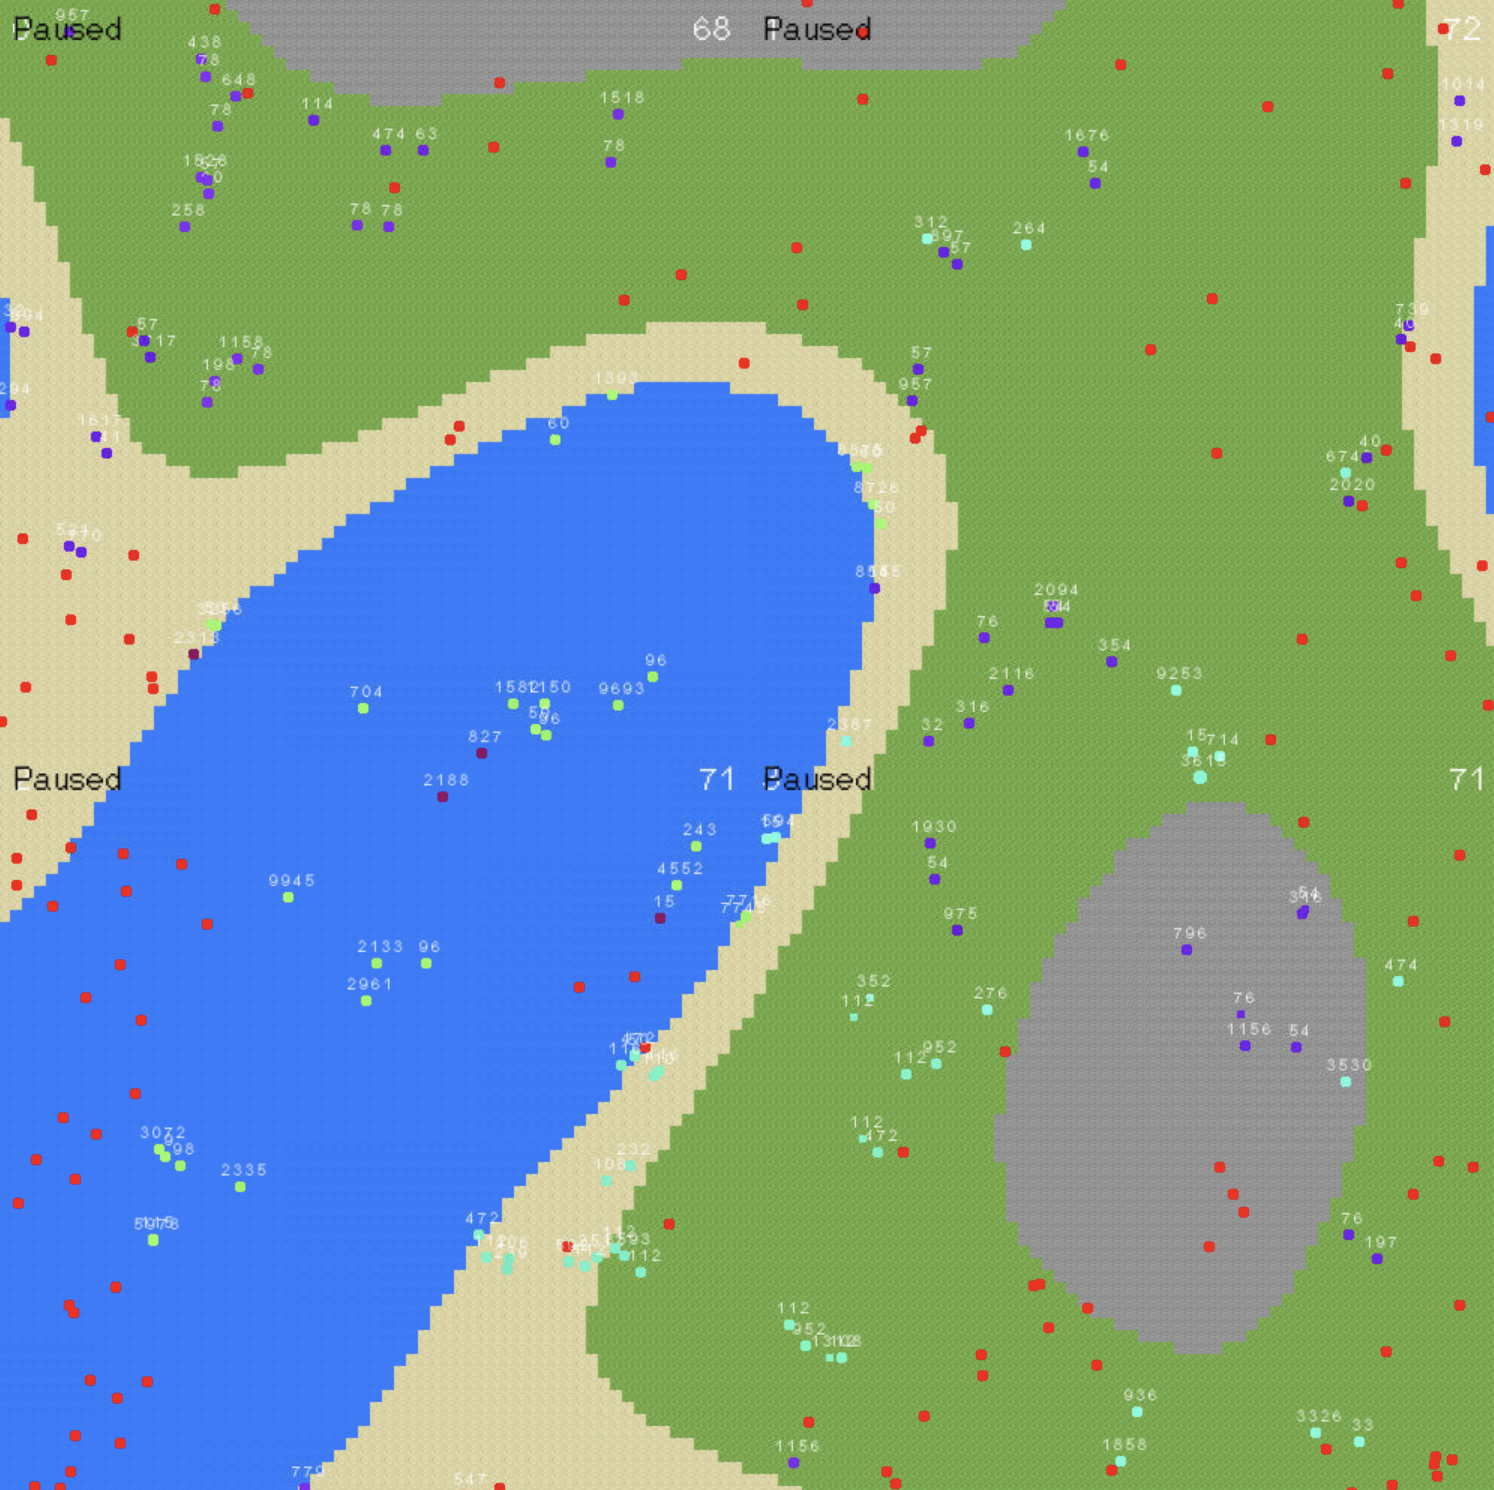
\includegraphics[width=\textwidth]{res/ergebnisse-simulation-2.png}
    \caption{Beispielhafter Ausschnitt der Simulation (2)}
    \label{fig:ergebnisse-simulation-2}
\end{figure}

\begin{figure}
    \centering
    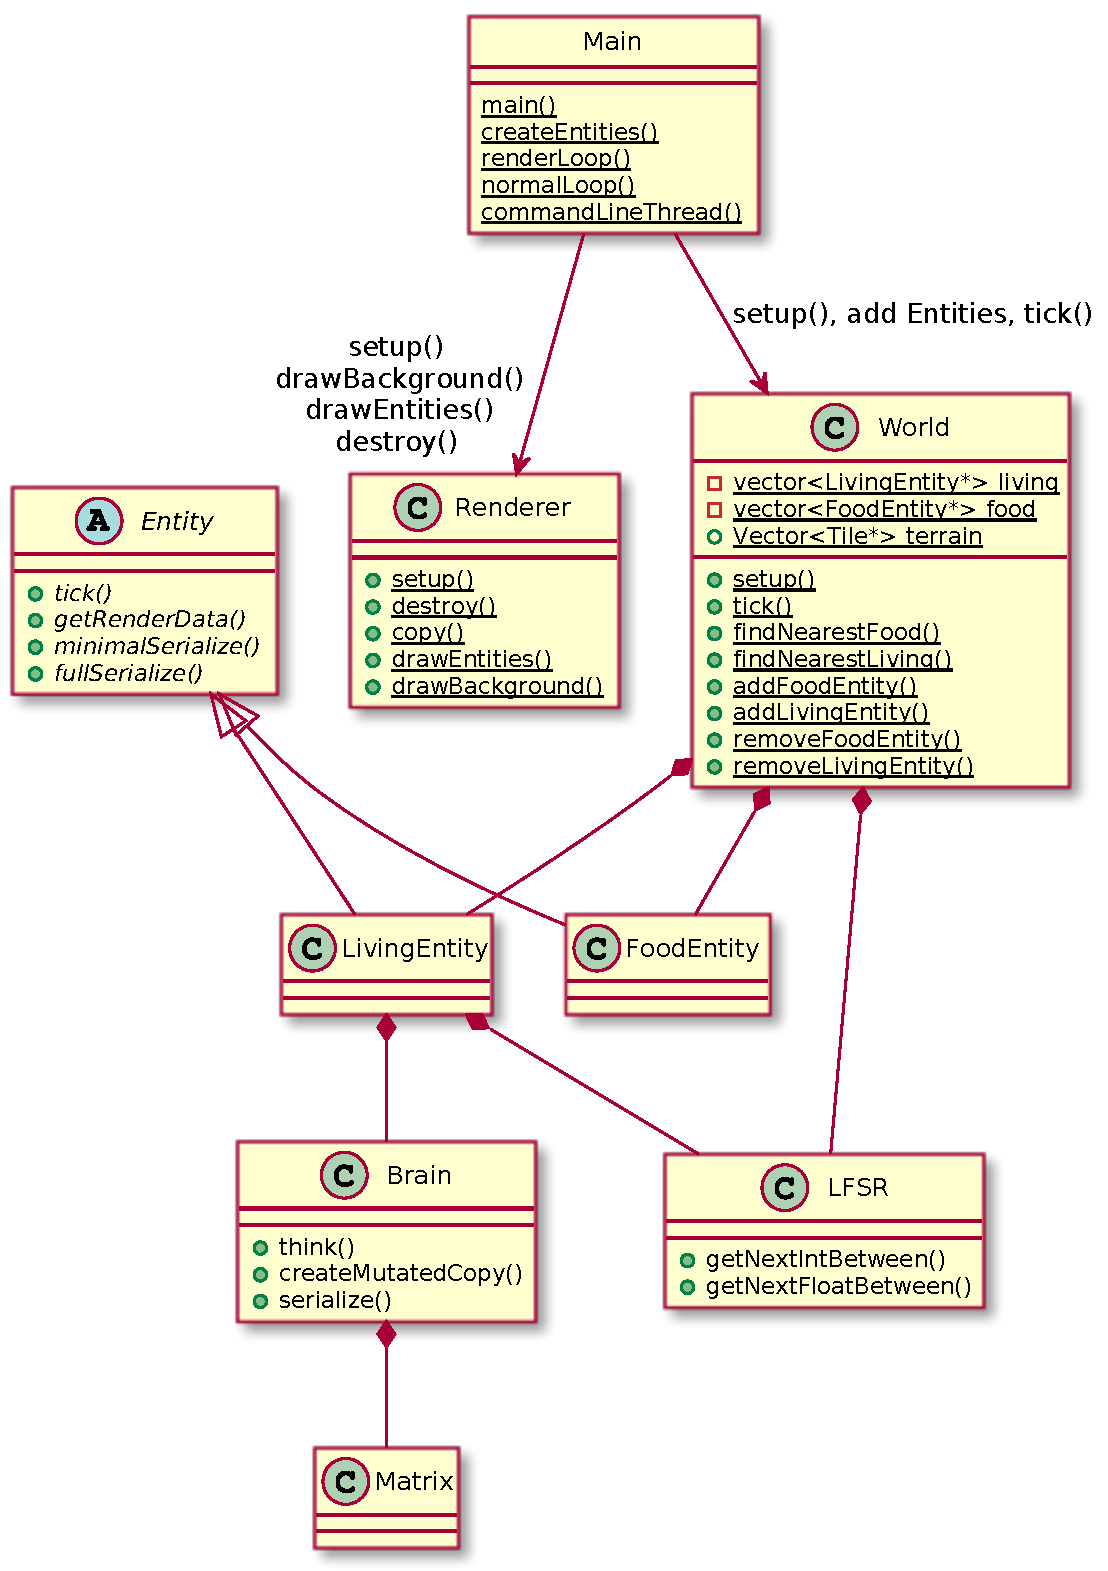
\includegraphics[width=\textwidth]{res/overview.pdf}
    \caption{Überblick über die Struktur}
    \label{fig:class-overview}
\end{figure}

\newpage
\begin{figure}
\centering
\begin{longtable}{| p{2cm} | p{12cm} |}
\hline
Parameter & Beschreibung \\
\hline
\hline
-w & Legt die \textbf{Breite} der gesamten Welt in Pixeln fest. Standardwert sind 1000px.\\
\hline
-h & Legt die \textbf{Höhe} der gesamten Welt in Pixeln fest. Standardwert sind 1000px.\\
\hline
-f & Gibt die Geschwindigkeit, mit welcher \textbf{neue \emph{FoodEntity}s} erscheinen sollen an. Die Einheit ist hier ein Entity pro 2000 \emph{Tiles} pro Tick. Gültige Werte sind positive Dezimalzahlen, der Standardwert ist 0.2.\\
\hline
-t & Soll die Ausführung nach einer bestimmten Anzahl an Ticks automatisch beendet werden, so kann dies hier spezifiziert werden. Übergeben wird die \textbf{Anzahl der auszuführenden Ticks}. Der Standardwert -1 bricht das Programm nicht automatisch ab.\\
\hline
-r & Standardmäßig wird die Simulation nicht \textbf{visuell dargestellt}. Dies lässt sich - sofern das Programm zum Rendern kompiliert ist - ändern, indem dieser Parameter ohne Wert übergeben wird. Alternativ kann das rendern auch jederzeit interaktiv aktiviert werden (siehe \ref{sssec:interact-console})\\
\hline
-z & Mit Hilfe einer positiven Dezimalzahl, deren Wert 0.1 nicht unterschreiten darf wird hier die \textbf{Vergrößerung} der Hintergrundkarte festgelegt. Größere Zahlen bedeuten also weniger und dafür größere Bereiche wie Wasser oder Berge. Der Standardwert ist 3.\\
\hline
-m & Dieser Parameter ermöglicht die Ausführung auf dem \textbf{MaiMUC}. Er legt die Größe der Welt und der jeweiligen Knoten passend zu den Bildschirmen den MaiMUC fest und sorgt dafür, dass der richtige Teil der Welt auf dem richtigen Display erscheint. Die Ausführung ist nur mit genau 10 MPI Nodes möglich.\\
\hline
-s & Um eine möglichst deterministische Messung zu ermöglichen, kann hier ein \textbf{Seed} für die Generierung der Zufallszahlen festgelegt werden. Wird dieser Parameter nicht angegeben, so wird zufällig initialisiert.\\
\hline
-e & Die \textbf{Anzahl der Entities}, die zu Beginn der Simulation auf die komplette Welt verteilt werden sollen. Das Format hierfür ist \emph{-e<Anzahl der LivingEntitys>,<Anzahl der FoodEntitys>}. Der Standardwert ist 500,500.\\
\hline
-p & Wird die Welt angezeigt, so kann mittels dieses Parameters ein Limit für die maximale Anzahl an \textbf{Ticks pro Sekunde} angegeben werden. Dieses Limit besteht, um eine realistischere Darstellung der aktuellen Ereignisse zu gewährleisten, bei welcher beispielsweise die Geschwindigkeit der Entities nicht von der Rechengeschwindigkeit abhängt. Der Standardwert 10 limitiert die Simulation auf maximal 10 Ticks pro Sekunde, durch Angabe des Wertes 0 kann die Beschränkung deaktiviert werden.\\
\end{longtable}
\end{figure}

\begin{figure}
\centering
\begin{longtable} {| p{2cm} | p{12cm} |}
\hline
-l & Dieser Parameter ermöglicht es, eine\textbf{Logdatei} von der Ausführung im CSV Format zu speichern.
Es muss der Anfang des Dateinamens übergeben werden, wobei sich der Tatsächliche Name ergibt durch \emph{<angegebener Name>-<MPI\_Rank>.csv}.\\
\hline
-o & Legt die Anzahl an \textbf{Threads} fest, die für die Ausführung verwendet werden sollen. Standardwert ist 1 (nur ein Master-Thread).\\
\hline
-b & Durch Angabe dieses Parameters ohne Wert kann der "`\textbf{boarisch}"' Modus aktiviert werden. Anstelle von roten Punkten wird Nahrung nun als Brezen dargestellt. Darüber hinaus wird bei einem Mausklick (siehe \ref{sssec:interact-render}) statt normaler Nahrung Bier erzeugt. Wird dieses gefressen, so wird das Living-Entity "`betrunken"'. Seine Bewegung wird für die nächsten Ticks mit der Sinuskurve interpoliert, wobei die Gewichtung stetig abnimmt, bis es wieder "`nüchtern"' ist.\\
\hline
\end{longtable}
\caption{Parameter, die beim Start der Ausführung übergeben werden können, um die Konfiguration der Simulation anzupassen}
\label{table:parameters}
\end{figure}


\begin{figure}
\centering
\begin{longtable}{| p{2cm} | p{12cm} |}
\hline
Aktion & Wirkung \\
\hline
\hline
Linksklick / Berührung &
An der entsprechenden Stelle wird Nahrung erzeugt. Im "`boarisch"' Modus (siehe \ref{sssec:exec-params}) handelt es sich hierbei um Bier, ansonsten um normale Nahrung. \\
\hline
Rechtsklick &
Die Attributwerte des nächstgelegenen \emph{LivingEntity}s werden auf der Konsole ausgegeben. \\
\hline
P &
Mit Hilfe dieser Taste kann die komplette Simulation pausiert und durch erneutes Drücken wieder fortgesetzt werden.\\
\hline
S &
Diese Taste aktiviert den "`Ähnlichkeitsmodus"', welcher durch erneutes Drücken verlassen werden kann. Die Simulation wird auch hier pausiert. Werden nun zwei \emph{LivingEntity}s nacheinander mit Rechtsklick angeklickt, so wird deren Unterschied, welcher über die Zugehörigkeit zur gleichen oder einer anderen Spezies entscheidet, auf der Konsole ausgegeben.\\
\hline
B &
Zeigt eine rote Umrandung um jeden Teil der Welt, welcher von einem eigenen Knoten verwaltet wird. Dies kann insbesondere bei der Ausführung mehrerer MPI-Knoten auf einem Gerät hilfreich sein.\\
\hline
A &
Analog können hier die Bereiche eines Knotens, welche auch auf anderen Knoten vorhanden sind angezeigt werden.\\
\hline
H &
Um die Simulation schnell in einem weiter fortgeschrittenen Stadium zu sehen, kann das Rendern hier zwischenzeitlich deaktiviert werden, wodurch ein deutlich schnellerer Ablauf ermöglicht wird. Zur Reaktivierung der Anzeige muss die Konsole verwendet werden (siehe \ref{sssec:interact-console}).\\
\hline
Q &
Beendet die Simulation endgültig.\\
\hline
\end{longtable}
\caption{Mögliche Interaktionen mit der Simulation über das Fenster}
\label{table:interact-window}
\end{figure}

\end{document}
